\documentclass[openright, dottedtoc, headinclude, footinclude=true, a4paper, numbers=noenddot, fontsize=10pt]{scrreprt}
\usepackage[eulermath, pdfspacing]{classicthesis}

\title{Nondeterministic Concurrency in Pure Functional Languages}
\author{Michael Walker}
\date{January 2016}

% Headings
\usepackage{titlesec}
\titlespacing{\section}{0pt}{0.5\baselineskip}{0.5\baselineskip}
\titlespacing{\paragraph}{0pt}{0.3\baselineskip}{1em}
\titleformat{\paragraph}[runin]{\normalfont\normalsize}{\theparagraph}{0pt}{\textbf}
\renewcommand{\descriptionlabel}[1]{\hspace*{\labelsep}\textbf{#1}}

% Nicer fonts
\usepackage[T1]{fontenc}
\usepackage{lmodern}

% Hyperlinks, URLs etc.
\usepackage{hyperref}
\usepackage{color}
\usepackage{url}
\hypersetup{
 colorlinks,
 citecolor=red,
 linkcolor=black,
 urlcolor=blue
}

% Figures
\usepackage{float}
\usepackage{caption}
\usepackage{subcaption}
\usepackage{caption}
\usepackage{placeins}
\usepackage{pgfgantt}

\DeclareCaptionFormat{underlined}{#1#2#3\hrulefill}
\captionsetup[figure]{format=underlined}

\DeclareCaptionFormat{normal}{#1#2#3}
\captionsetup[subfigure]{format=normal}

% Listings
\usepackage{minted}
\usemintedstyle{trac}
\newminted{haskell}{}
%TC:group minted [ignore] xall

% Footnotes
\renewcommand{\thefootnote}{\fnsymbol{footnote}}
\usepackage{perpage}
\MakePerPage{footnote}

% Citations & Quotes
\usepackage[square]{natbib}

% Definitions

\newcommand{\defineword}[2]{%
\begin{description}%
    \item{\textbf{#1}} \hfill \\%
        {#2}%
\end{description}%
}

\newcommand{\definewordc}[3]{%
\begin{description}%
    \item{\textbf{#1}} \citep{#2}\hfill \\%
        {#3}%
\end{description}%
}

% Page layout jiggery pokery
\usepackage[top=3cm,bottom=3cm]{geometry}

% Front/main matter
\newcommand{\frontmatter}{\cleardoublepage\pagenumbering{roman}}
\newcommand{\mainmatter}{\cleardoublepage\pagenumbering{arabic}}

% Appendices
\usepackage{pdfpages}

% Misc
\newcommand{\quot}[2]{``\textit{#1}''\cite{#2}}
\newcommand{\sect}[1]{\S\ref{sec:#1}}
\newcommand{\chap}[1]{Chapter \ref{chp:#1}}
\newcommand{\todo}[1]{\textcolor{red}{TODO: #1}}
\newcommand{\dejafu}{D\'{e}j\`{a} Fu}

\begin{document}

\frontmatter

\begin{titlepage}
\begin{center}

\includegraphics{university-of-york.eps}\\[2em]

\hrule
\vspace{1em}

{\huge\bfseries Nondeterministic Concurrency in Pure Functional Languages}\\[1em]

\hrule
\vspace{1em}

{\normalsize Progress Report for Ph.D Computer Science}\\[0.5cm]

{\small \textsc{Author:} Michael Walker, \textsc{Supervisor:} Colin Runciman}\\[0.5cm]

\normalsize{Department of Computer Science\par
University of York}\\[0.25cm]

\small{January 2016}
\end{center}

\vspace{2cm}

\centerline{\rule{40pt}{1pt} \textsc{\large Abstract} \rule{40pt}{1pt}}
\vspace{0.1cm}

This interim report discusses developments and new research directions
since the qualifying dissertation. The scope of the work is improving
the ease of writing correct concurrent functional programs, and is
being done in the context of Haskell.

The \dejafu{} tool for testing concurrent Haskell programs has had
significant development: support for relaxed memory models; use of
partial-order reduction over schedule bounding; and more supported
operations.

Research directions for the future are identified. These are:
submitting a journal article detailing the updated \dejafu{} tool; LTL
property checking; the automated generation of properties of
concurrent programs, suitable for use as test cases; the automated
parallelisation of list comprehensions; and the encoding of safety
properties as types.


\vfill
\begin{center}
Number of words: 4122 as counted by ``texcount -inc'',\\
excluding code listings.  
\end{center}
\end{titlepage}

\tableofcontents

%\listoffigures
%\listoftables
%\lstlistoflistings

\mainmatter

\chapter{Introduction}
\label{chp:intro}
This chapter describes the test execution of a concurrent program
written using the \verb|MonadConc| abstraction, not the execution of
programs using GHC's actual concurrency primitives. Of course, for
correctness of testing, there should be a correspondence between these
two models, see \chap{correctness}.

The execution of a concurrent program is considered to be the
sequential stepwise execution of \emph{primitive actions}, the most
basic things that a computation can do.


  \section{Scope}
  \label{sec:intro-scope}
  We aim to support all of the functionality of GHC's concurrency API
which does not unavoidably \emph{require} support from the runtime,
and which is not so nondeterministic that there is no sensible way to
model it accurately.

Some specific examples of things which are out of scope:

\begin{itemize}
\item \verb|threadDelay|, as all this guarantees is that a thread will
  not run \textit{sooner} than the delay. There is no upper bound on
  the delay, and also no guarantee that any other thread will be
  scheduled during the delay.

\item \verb|threadWaitRead|, \verb|threadWaitWrite|, and the
  \verb|STM| variants, as there is no way to tell if a file descriptor
  can be read from or written to without involving \verb|IO|, and in
  addition this is influenced by other non-Haskell processes accessing
  the same file.

\item Bound threads, as these affect which operating system thread FFI
  calls operate on, and so alters program behaviour in a parallel
  setting.

\item \verb|BlockedIndefinitely| exceptions, as this is a garbage
  collection problem, which is out of the reach of the runtime. There
  are some annotation functions to record which shared state a thread
  knows about, and so this can be supported on a limited scale, but
  not even GHC makes any guarantee of it being reliable.\footnote{
    \quot{Note that this feature is intended for debugging, and should
      not be relied on for the correct operation of your
      program. There is no guarantee that the garbage collector will
      be accurate enough to detect your deadlock, and no guarantee
      that the garbage collector will run in a timely enough
      manner.}{controlConcurrent}}
\end{itemize}


\chapter{Progress Review}
\label{chp:progress}
This chapter describes the test execution of a concurrent program
written using the \verb|MonadConc| abstraction, not the execution of
programs using GHC's actual concurrency primitives. Of course, for
correctness of testing, there should be a correspondence between these
two models, see \chap{correctness}.

The execution of a concurrent program is considered to be the
sequential stepwise execution of \emph{primitive actions}, the most
basic things that a computation can do.


  \section{\dejafu{}: A Concurrency Testing Library for Haskell}
  \label{sec:progress-dejafu}
  \begin{displayquote}
  % hack to stop the displayquote from eating the [
  {[}\dejafu{} is] A martial art in which the user's limbs move in
  time as well as space, [\ldots] It is best described as ``the
  feeling that you have been kicked in the head this way
  before.'' \parencite{pratchett2001}
\end{displayquote}

\noindent
Specialised tools are necessary to test concurrent programs.  In this
chapter we present and evaluate \dejafu{}, our library for testing
concurrency in Haskell.  We discuss the scope of the
tool~\sref{dejafu-scope} and present our abstraction over the GHC
Haskell concurrency functionality~\sref{dejafu-monadconc}.  We then
show an example of a small logic puzzle which we can represent as a
concurrent program~\sref{dejafu-100}.  We explain how programs using
our abstraction are executed~\sref{dejafu-execution}, and give our
semantic rules~\sref{dejafu-semantics}.  We explain how we test
programs~\sref{dejafu-testing}, and argue the correctness of the
testing approach~\sref{dejafu-correctness}.  We present three case
studies~\sref{dejafu-casestudies}, and finally evaluate our
results~\sref{dejafu-evaluation}.

This chapter is derived from our previous work \cite{walker2015} and
\cite{YCS-2016-503}.

\section{What is \dejafu{}?}
\label{sec:dejafu-whatis}

\dejafu{} is a tool for testing concurrent Haskell programs.  It works
by providing a typeclass abstraction over the concurrency operations
of interest, called \verb|MonadConc|, and using an implementation of
this class based on inspectable continuations to explore the
nondeterministic behaviours of a program under test.

\begin{listing}
\centering
\begin{cminted}{haskell}
runSCTWithSettings :: MonadConc m
  => Settings m a
  -> ConcT m a
  -> m [(Either Failure a, Trace)]
\end{cminted}
\caption{The core API of \dejafu{}.}\label{lst:dejafucore}
\end{listing}

\Cref{lst:dejafucore} gives the type signature of the function at the
heart of \dejafu{}.  The first parameter is configuration, controlling
how \dejafu{} explores the space of executions.  The second is the
concurrent program to test: \verb|ConcT m| is \dejafu{}'s
implementation of \verb|MonadConc|, it is parameterised by some monad
\verb|m| which is used to provide mutable variables.  Typically this
\verb|m| will be \verb|IO|.  The function returns a collection of
tuples.

The outputs which \dejafu{} produces are pairs, where the first
component is the result of the program and the second is the execution
trace which led to it.  A program may not complete successfully: it
may deadlock or throw an exception in the main thread which does not
get caught.  If the program does complete successfully, the first
component of the tuple will be a \verb|Right| containing the actual
value produced, otherwise it will be a \verb|Left| and the
\verb|Failure| value will show what went wrong.  A \verb|Trace| is a
list of scheduling decisions, with a summary of what the chosen thread
did in that step of execution.

In outline, \verb|runSCTWithSettings| works like so:

\begin{enumerate}
\item Repeat until there are no more executions:
  \begin{enumerate}
  \item Set up the initial state, where only the main thread exists
  \item While the main thread exists, and there are runnable threads:
    \begin{enumerate}
    \item Choose a thread
    \item Run the next action in that thread
    \end{enumerate}
  \item Add the result pair to the output
  \end{enumerate}
\end{enumerate}

We produce different schedules by maintaining some state, and using
that when choosing threads.  \dejafu{} supports three ways to explore
the behaviours of a concurrent program:

\begin{description}
\item[Randomly] Threads are chosen using a uniform random
  distribution.  Exploration terminates after a fixed number of
  executions.

\item[Swarm] Threads are chosen using a weighted random distribution.
  Exploration terminates after a fixed number of executions.  We
  discuss this algorithm further in \Cref{chp:algorithms}.

\item[DPOR] Uses a notion of ``todo sets,'' where each
  scheduling point has an associated set of threads to try in future
  executions.  Execution terminates when all such sets are empty.

  During execution, at each scheduling point, if the previously chosen
  thread is still runnable, choose that; otherwise, take all runnable
  threads, choose one arbitrarily, and record the others in the todo
  set for this scheduling point.

  After execution, the trace is examined to find pairs of dependent
  actions: for each thread $T$, for each action in thread $T$, find
  the most recent dependent action (if one exists) in a different
  thread, and add $T$ to the todo set corresponding to that scheduling
  point if $T$ is runnable; otherwise add all runnable threads.

  There are some subtleties and additional optimisations, which we
  discuss further in \Cref{sec:dejafu-testing}.
\end{description}

\dejafu{} tests use predicates on the list of result pairs.  These
predicates can check anything, for example all results being
\verb|Right|s and equal.  To remove result pairs that we don't want a
predicate to examine, \dejafu{} supports ``online'' filtering, where
such pairs are discarded as they are found.  This is configured in the
\verb|Settings| value.

\paragraph{Scope}
We aim to support most of the functionality of GHC’s concurrency API.
However, some operations are more trouble than they're worth: for
example, operations which introduce additional sources of
nondeterminism, or which unavoidably require support from the runtime
system.  In particular, we do not support:

\begin{itemize}
\item Operations to block a thread until a file descriptor becomes
  available, as this introduces an additional source of
  nondeterminism.

\item Operations to query which capability (OS thread) a Haskell
  thread is running on, as this introduces an additional source of
  nondeterminism.

\item Automatically detecting if a thread is deadlocked on an
  \verb|MVar| or \verb|TVar| and throwing an exception to it, as we
  cannot detect this situation without support from the garbage
  collector.
\end{itemize}

We also do not yet support \emph{bound threads}: a Haskell thread
which will always run on the same, unique, OS thread.  Bound threads
are essential for using the foreign function interface (FFI) to call C
libraries which use thread-local state, to ensure the Haskell thread
always sees its state and never the state of another thread.  We have
a prototype implementation, which is planned to be included in the
next major release of
\dejafu{}\footnote{\url{https://github.com/barrucadu/dejafu/issues/126}}.

\paragraph{Semantic departures}
In the functionality we do support, we model behaviour as close as
reasonably possible to GHC.  We make a few departures from the
traditional semantics where there is good reason to do so:

\begin{itemize}
\item Runtime errors, such as pattern match failures, can be caught as
  exceptions inside \verb|IO|.  As there is no non-\verb|IO| way to do
  the same, \dejafu{} cannot catch these errors.

\item We do not model threads delaying, and implement any delays as
  yields.  It is not clear how to incorporate time into the testing
  model.
\end{itemize}

\paragraph{Embedded \texttt{IO} actions}
\dejafu{} supports testing computations with embedded \verb|IO|
actions provided that the programmer ensures that the action is
atomic; that it is deterministic when executed with a fixed schedule;
and that it does not block on the action of another thread.  Failing
to meet any of these conditions may lead to incomplete testing.

\section{Abstracting over Concurrency}
\label{sec:dejafu-monadconc}

There are three ways of implementing a concurrency testing tool:
overriding the concurrency primitives of the language; instrumenting
the source program; or instrumenting the compiled program.  We adopt
the first approach in \dejafu{}.  Haskell's typeclass machinery lets
us specify an interface for concurrency, and to provide different
concrete implementations.  There is one implementation using the
\verb|IO| type and the standard functions; there is another using our
own type, based on continuations which we can inspect.

\begin{listing}
\centering
\begin{cminted}{haskell}
class (Monad m, {- other constraints omitted -}) => MonadConc m where
  type MVar m :: * -> *
  -- other types omitted

  newEmptyMVar :: m (MVar m a)
  newEmptyMVar = newEmptyMVarN ""

  newEmptyMVarN :: String -> m (MVar m a)
  newEmptyMVarN _ = newEmptyMVar

  putMVar  :: MVar m a -> a -> m ()
  readMVar :: MVar m a -> m a
  takeMVar :: MVar m a -> m a
  -- other operations omitted
\end{cminted}
\caption{A fragment of the \texttt{MonadConc} typeclass.}\label{lst:monadconc}
\end{listing}

We call our typeclass \verb|MonadConc|: monads which do concurrency.
\Cref{lst:monadconc} shows a fragment.  To define an instance, the
programmer supplies concrete types for the abstract types and
implementations of all undefined operations.  Some operations have
default definitions: for example, there are two ways of constructing
an empty \verb|MVar|.  One way takes a name, which is displayed in
debugging information, the other does not.  Each has a default
definition in terms of the other, so the programmer must supply at
least one.

\begin{listing}
\centering
\begin{cminted}{haskell}
instance Monad n => MonadConc (ConcT r n) where
  type MVar (ConcT r n) = ModelMVar r
  -- other types omitted

  newEmptyMVarN n = toConc (ANewMVar n)

  putMVar  var a = toConc (\c -> APutMVar var a (c ()))
  readMVar var   = toConc (AReadMVar var)
  takeMVar var   = toConc (ATakeMVar var)
  -- other operations omitted
\end{cminted}
\caption{A fragment of the \texttt{MonadConc} testing implementation.}\label{lst:mvarops}
\end{listing}

The type for our testing implementation is called \verb|ConcT r n|,
which is a monad that has access to references of type \verb|r| in a
monad of type \verb|n|.  \Cref{lst:mvarops} shows a fragment of the
instance of \verb|MonadConc| for this type.  Each concurrency
operation is of the same form: we take the arguments and wrap them up
inside a data structure whose final argument is a continuation, which
is then converted into a \verb|ConcT| value.

We represent a concurrent computation as a large value.  We can
inspect each step of the computation by looking at the data
constructor used.  We call these constructors \emph{primitive
  actions}.  With these actions we express the operations in the
\verb|MonadConc| class.

\section{The $n$ Prisoners Problem}
\label{sec:dejafu-100}

\begin{displayquote}
  There are $n$ prisoners in solitary cells.  There's a central living
  room with one light bulb.  No prisoner can see the light bulb from
  their own cell.  Every day, the warden picks a prisoner equally at
  random, and that prisoner visits the living room.  While there, the
  prisoner may toggle the bulb.  The prisoner also has the option of
  asserting that all $n$ prisoners have been to the living room.  If
  this assertion is false, all $n$ prisoners are shot.  However, if
  true, all prisoners are set free.  Thus, the assertion should only
  be made if the prisoner is 100\% certain of its validity.  The
  prisoners are allowed to get together one night in the courtyard, to
  discuss a plan.  What plan should they agree on, so that eventually,
  someone will make a correct assertion?
\end{displayquote}

We can express this puzzle as a concurrency problem: the warden is the
scheduler, each prisoner is a thread, and when the program terminates
every prisoner should have visited the living room.  So if every
thread (prisoner) is scheduled (taken to the room), the prisoners are
successful.  \dejafu{} can give us execution traces.  So, given some
way of setting up the prison, we can use \dejafu{} to execute it and
then examine the returned traces to discover if the prisoners are
successful.

\subsection{The Probabilistic Solution}

One school of thought says to just wait for $10 n$ days, because by
then it's unlikely that any prisoner has not visited the room.  The
chance that any one prisoner will have been consistently missed is
$\left(1 - \frac{1}{n}\right)^{10n}$, which converges to
$\frac{1}{e^{10}}$.

\Cref{lst:100good} shows an implementation of this strategy, and
\Cref{tbl:100rand} shows how the prisoners fare over 100 random
executions.  We see that the number of room visits grows a little
faster than ten for each additional prisoner, this is because of a
quirk of our implementation.  We have nominated one prisoner to be the
leader, who is the only prisoner able to declare that all have visited
the room.  So our implementation ends up waiting $10 (n - 1)$ days for
the non-leaders to visit, and then however many days it takes for the
leader to visit after that.

\begin{table}
  \centering
  \begin{tabular}{lrrrrrrrr} \toprule
    Prisoners          &   1 &   2    &   3    &   4    &   5    &   6    &   7    &   8 \\
    Successes          & 100 & 100    & 100    & 100    & 100    & 100    & 100    & 100 \\
    Failures           &   0 &   0    &   0    &   0    &   0    &   0    &   0    &   0 \\
    Avg.\@ Room Visits &   2 &  18.35 &  31.92 &  43.52 &  55.88 &  67.37 &  77.05 &  90.40 \\ \bottomrule
  \end{tabular}
  \caption{The behaviour of the probabilistic solution.}\label{tbl:100rand}
\end{table}

\subsection{The Perfect Solution}

Perhaps our prisoners are more cautious, and even a small chance of
death is too much.  They want to be certain of their success.  A slow
but simple strategy is for the prisoners, like in our probabiistic
solution, to nominate a leader.  Only the leader can declare to the
warden that everyone has visited the room.  Whenever a prisoner other
than the leader visits the room, if this is their first time in the
room with the light off, they turn it on, otherwise they do nothing.
Whenever the leader enters the room, they turn the light off.  When
the leader has turned the light off $n-1$ times, they tell the warden
that everyone has visited.  \Cref{lst:100perfect} shows an
implementation of these behaviours.

\begin{listing}
\begin{sublisting}{\textwidth}
\centering
\begin{cminted}{haskell}
leader :: MonadConc m => Int -> TVar (STM m) Int -> m ()
leader numPrisoners days = atomically $ do
  numDays <- readTVar days
  when (numDays < (numPrisoners - 1) * 10) retry

notLeader :: MonadConc m => TVar (STM m) Int -> m ()
notLeader days = forever $ atomically (modifyTVar days (+1))

prison :: MonadConc m => Int -> m ()
prison numPrisoners = do
  days <- atomically (newTVar 0)
  for_ [1..numPrisoners-1] (\_ -> fork (notLeader days))
  leader numPrisoners days
\end{cminted}
\caption{The probabilistic solution: just wait a long time and gamble.}\label{lst:100good}
\end{sublisting}

% [layout hack]: no gap between the listings otherwise
\vspace{1.5em}

\begin{sublisting}{\textwidth}
\centering
\begin{cminted}{haskell}
data Light = IsOn | IsOff

leader :: MonadConc m => Int -> TVar (STM m) Light -> m ()
leader numPrisoners light = go 0 where
  go counter = do
    counter' <- atomically $ do
      state <- readTVar light
      case state of
        IsOn -> do
          writeTVar light IsOff
          pure (counter + 1)
        IsOff -> retry
    when (counter' < prisoners - 1)
      (go counter')

notLeader :: MonadConc m => TVar (STM m) Light -> m ()
notLeader light = do
  atomically $ do
    state <- readTVar light
    case state of
      IsOn  -> retry
      IsOff -> writeTVar light IsOn
  forever yield

prison :: MonadConc m => Int -> m ()
prison numPrisoners = do
  light <- atomically (newTVar IsOff)
  for_ [1..numPrisoners-1] (\_ -> fork (notLeader light))
  leader numPrisoners light
\end{cminted}
\caption{The perfect solution: nominate a leader, who waits until they are certain that everyone has been in the room.}\label{lst:100perfect}
\end{sublisting}
\caption{Two solutions for the $n$ prisoners problem.}\label{lst:100sols}
\end{listing}

We can satisfy ourselves that this solution works for all cases by
using \dejafu{}'s systematic concurrency testing functionality, which
is a combination of dynamic partial-order reduction and schedule
bounding.  \Cref{tbl:100slow} shows how the number of schedules
explored and average number of room visits grows as the number of
prisoners increases.  It does not scale well.

This algorithm is something of a worst-case for DPOR.  Every thread is
modifying the same shared state, so DPOR has to try every
interleaving.  Taking another look at our prisoners, we can see two
things which a human would use to decide whether some schedules are
redundant or not:

\begin{table}
\begin{subtable}{\textwidth}
  \centering
  \begin{tabular}{lrrr} \toprule
    Prisoners          & 1 & 2 &    3 \\
    Schedules          & 1 & 5 & 2035 \\
    Avg.\@ Room Visits & 2 & 7 &  133 \\ \bottomrule
  \end{tabular}
  \caption{Using \dejafu{}'s default schedule bounds.}\label{tbl:100slow}
\end{subtable}

% [layout hack]: no gap between the tables otherwise
\vspace{1.5em}

\begin{subtable}{\textwidth}
  \centering
  \begin{tabular}{lrrrrrr} \toprule
    Prisoners          & 1 & 2 & 3   &  4   &    5 &      6 \\
    Schedules          & 1 & 1 & 4   & 48   & 1536 & 122880 \\
    Avg.\@ Room Visits & 2 & 4 & 7.5 & 11.5 &   16 &     21 \\ \bottomrule
  \end{tabular}
  \caption{Using a custom fair bound to prevent yields.}\label{tbl:100fast}
\end{subtable}
\caption{How the number of schedules grows with increasing prisoner numbers.}\label{tbl:100slowfast}
\end{table}

\begin{enumerate}
\item If we adopt any schedule other than alternating leader /
  non-leader, threads will block without doing anything.  So we should
  alternate.
\item When a non-leader has completed their task, they will always
  yield.  So we should never schedule a prisoner who will yield.
\end{enumerate}

\dejafu{} cannot make use of (1).  However, it would be possible to
implement this optimisation if \dejafu{} were able to compare values
inside \verb|TVar|s.  We would then be able to check if any
\verb|TVar| read during a transaction which blocked has a different
value: if none do, the transaction will just block again.  But we
cannot do that without putting an \verb|Eq| constraint on
\verb|writeTVar|, so this would require a new primitive action.  We
get part of the way there, though.  If a thread is blocked in a
transaction, \dejafu{} only tries executing it again when at least one
of the \verb|TVar|s it reads from has been written to, which gives a
similar effect to the version numbering scheme commonly used in STM
implementations \parencite{shavit1995}.

\dejafu{} can make use of (2).  \dejafu{} already bounds the maximum
number of times a thread can yield, so that it can test constructs
like spinlocks.  This is called \emph{fair bounding}.  The default
bound is five, but if we set it to zero \dejafu{} will never schedule
a thread which is going to yield.  \Cref{tbl:100fast} shows how the
number of schedules explored and average number of room visits grow
with this change.

This is better, but still scales poorly.  The program is still a bad
case for DPOR.  This is probably as good as we can do without adding
some extra primitives to \dejafu{} to optimise the case where we have
an \verb|Eq| instance available, or by using an alternative systematic
testing algorithm.  In \Cref{chp:algorithms} we will discuss an
alternative \emph{incomplete} approach to this, and other, concurrency
problems.

It's not the end for DPOR, however.  Empirical
studies \parencite{thomson2014} have found that many concurrency bugs can be
exhibited with only two or three threads.  Furthermore, most
real-world concurrent programs do not have every single thread
operating on the same bit of shared state.  So in practice, we will
tend not to see this exponential growth in schedules tried.

\section{Executing Concurrent Programs}
\label{sec:dejafu-execution}

We represent operations in the \verb|MonadConc| typeclass by the
\verb|Action| type.  Each action describes some effect and contains a
continuation.  A concurrent computation is a sequence of these
continuation values.  Each thread is terminated by a distinguished
\emph{stop} primitive, which has no continuation.

% [layout hack]: get lst:100sols here
\FloatBarrier

\begin{listing}
\centering
\begin{cminted}{haskell}
newtype M n r a = M { runM :: (a -> Action n r) -> Action n r }

instance Functor (M n r) where
  fmap f m = M (\c -> runM m (c . f))

instance Applicative (M n r) where
  pure x  = M (\c -> AReturn (c x))
  f <*> v = M (\c -> runM f (\g -> runM v (c . g)))

instance Monad (M n r) where
  return  = pure
  m >>= k = M (\c -> runM m (\x -> runM (k x) c))

instance MonadFail (M n r) where
  fail e = M (\_ -> AThrow (MonadFailException e))
\end{cminted}
\caption{The \dejafu{} continuation monad.}\label{lst:m}
\end{listing}

\Cref{lst:m} gives the definition and typeclass instances of the
\dejafu{} continuation monad.  The \verb|Functor| instance allows
applying a function to the input of the continuation.  The
\verb|Applicative| instance allows injecting a pure value into the
\verb|M| type, by constructing a continuation which consumes this
value.  It also allows extracting a function from one computation, a
value from another, and applying them.  The \verb|Monad| instance
allows sequencing.  Finally, the \verb|MonadFail| instance allows
signalling a pattern match failure in a monadic
expression\footnote{\dejafu{} aims to support the latest three major
  releases of GHC, so in the real implementation use conditional
  compilation.}.

\begin{listing}
\centering
\begin{cminted}{haskell}
pure id <*> v
  = M (\c -> AReturn (c id)) <*> v
  = M (\c -> runM (M (\c -> AReturn (c id))) (\g -> runM v (c . g)))
  = M (\c -> (\c -> AReturn (c id)) (\g -> runM v (c . g)))
  = M (\c -> AReturn ((\g -> runM v (c . g)) id))
  = M (\c -> AReturn (runM v (c . id)))
  = M (\c -> AReturn (runM v c))
 /= v
\end{cminted}
\caption{Expansion of the \texttt{Applicative} identity law.}\label{lst:areturn}
\end{listing}

\paragraph{Nonterminating executions}
\dejafu{} is only able to make scheduling decisions at the level of
primitive actions, which means that if evaluating a primitive action
does not terminate, \dejafu{} will hang.  As \Cref{lst:areturn} shows,
we deliberately break the \verb|Applicative| identity law, that
\verb|pure id <*> v = v| for all \verb|v|, to make some programs more
defined than they otherwise would be.

\begin{listing}
\centering
\begin{cminted}{haskell}
test = forever (pure "loop") where
  forever mx = mx >> forever mx
\end{cminted}
\caption{A simple non-terminating program.}\label{lst:forever}
\end{listing}

\Cref{lst:forever} shows a program which is made more defined by
breaking the law.  Neither \verb|>>| nor \verb|forever| correspond to
primitive actions, so they cannot be pre-empted.  If \verb|pure| did
not correspond to a primitive action either, then that expression
would cause \dejafu{} to loop forever as it tries to compute the
continuation.  This is an unhelpful result.  By breaking the laws and
introducing a way to interrupt the \verb|forever| computation,
\dejafu{} can instead report that trying to test this program exceeds
the execution length
limit\footnote{\url{https://github.com/barrucadu/dejafu/issues/27} and
  \url{issues/113}}.

\paragraph{Scheduling}
The choice of which thread to execute is made by a scheduler function,
which is supplied by the user.  The scheduler is called even if there
is only one runnable thread, to keep things simple.  A scheduler has
the type declared in \Cref{lst:scheduler}.  It is a stateful function
which is given the previous action and the runnable threads, which
possibly returns a thread to run.  If no thread is returned, the
computation is aborted.  Aborting is used in the implementation of
schedule bounding.  The state is used in the implementation of
partial-order reduction and random scheduling: in the former, the
state is a list of scheduling decisions; in the latter, the state is a
random number generator.

\begin{listing}
\centering
\begin{cminted}{haskell}
newtype Scheduler state = Scheduler
  { scheduleThread
    :: Maybe (ThreadId, ThreadAction)
    -> NonEmpty (ThreadId, Lookahead)
    -> state
    -> (Maybe ThreadId, state)
  }
\end{cminted}
\caption{The \dejafu{} \texttt{Scheduler} type.}\label{lst:scheduler}
\end{listing}

\paragraph{Success and failure}
When testing concurrent computations, we are interested in both
success and failure.  If a computation succeeds and returns a value,
we want to know that; if it enters a failure state such as deadlock,
we also want to know that.  The result of a single execution of the
program is a value of type \verb|Either Failure result|, where the
\verb|Failure| type is an enumeration of error conditions that
\dejafu{} can detect, and the \verb|result| type is the result in the
successful case.

\subsection{Software Transactional Memory}

Transactions allow the atomic execution of a sequence of operations
involving \verb|TVar|s, transactional variables.  Unlike operations on
\verb|IORef|s or \verb|MVar|s, transactions are composable and the
whole remains atomic.  We express transactions in a similar way to
concurrent programs: as a monad of continuations over a primitive
action type.  As \dejafu{} drives the execution of a concurrent
program, it is possible to have arbitrarily complex effects which
appear atomic to the program under test.

A transaction evaluates to some success value, an uncaught exception,
or an abort.  If successful, it may also mutate some transactional
variables as a effect; otherwise it does not.  If it evaluates to an
uncaught exception, we raise the exception in the thread performing
the transaction.  If it evaluates to an abort, we block the thread
performing the transaction until at least one \verb|TVar| read in the
transaction is mutated by another thread.

\subsection{Relaxed Memory}

There are three memory models supported in \dejafu{}:

\begin{description}
\item[Sequential Consistency] This model is the most intuitive.  A program
  behaves as a simple interleaving of the actions in different threads.  When an
  \texttt{IORef} is written to, that write is immediately visible to all
  threads.

\item[Total Store Order (TSO)] Each thread has a write buffer.  A thread sees
  its writes immediately, but other threads will only see writes when they are
  \emph{committed}, which may happen later.  Writes by the same thread are
  committed in program order.

\item[Partial Store Order (PSO)] A relaxation of TSO where each thread has a
  write buffer for each \verb|IORef|.  Writes to different \verb|IORef|s by the
  same thread are not necessarily committed in program order.
\end{description}

The default memory model for testing is TSO, as that most accurately
models the behaviour of modern x86 processors \parencite{owens2009}.  The
use of a relaxed memory model can require a much larger number of
schedules when \verb|IORef|s are shared between threads.

\paragraph{Write buffering}
We model relaxed memory by introducing buffers for thread writes.  When a thread
writes to an \verb|IORef|, the write is appended to its buffer.  When a thread
reads from an \verb|IORef|, it reads the value of the newest write in its buffer,
or the most recently committed value if the buffer is empty.  After a write is
committed, it is removed from its buffer.  Any non-empty buffer may have a write
committed, but only the oldest write in a buffer may be committed.  \Cref{fig:wb}
shows the arrangement of buffers for the three memory models in a system with
two threads and two \verb|IORef|s.

\begin{figure}
  \centering
  \begin{subfigure}{0.3\textwidth}
    \centering
    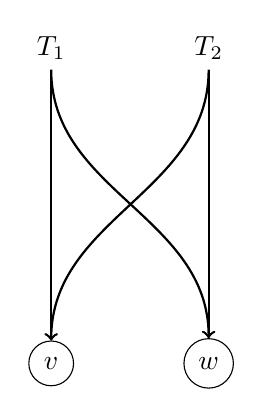
\begin{tikzpicture}
      \node (t1) at (-1,0) {$T_1$};
      \node (t2) at (1,0)  {$T_2$};
      \node (v) [draw,shape=circle] at (-1,-4) {$v$};
      \node (w) [draw,shape=circle] at (1,-4)  {$w$};

      \draw [->, thick] (t1.south) to [out=270,in=90] (v.north);
      \draw [->, thick] (t1.south) to [out=270,in=90] (w.north);
      \draw [->, thick] (t2.south) to [out=270,in=90] (v.north);
      \draw [->, thick] (t2.south) to [out=270,in=90] (w.north);
    \end{tikzpicture}
    \caption{Sequential Consistency}
  \end{subfigure}
  \begin{subfigure}{0.3\textwidth}
    \centering
    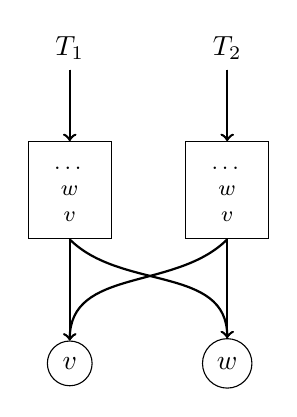
\begin{tikzpicture}
      \node (t1) at (-1,0) {$T_1$};
      \node (t2) at (1,0)  {$T_2$};
      \node (v) [draw,shape=circle] at (-1,-4) {$v$};
      \node (w) [draw,shape=circle] at (1,-4)  {$w$};

      \node (bt1) [draw] at (-1,-1.8) {\footnotesize\begin{tabular}{c} \ldots \\\midrule $w$ \\\midrule $v$ \end{tabular}};
      \node (bt2) [draw] at (1,-1.8) {\footnotesize\begin{tabular}{c} \ldots \\\midrule $w$ \\\midrule $v$ \end{tabular}};

      \draw [->, thick] (t1) to [out=270,in=90] (bt1);
      \draw [->, thick] (t1) to [out=270,in=90] (bt1);
      \draw [->, thick] (t2) to [out=270,in=90] (bt2);
      \draw [->, thick] (t2) to [out=270,in=90] (bt2);

      \draw [->, thick] (bt1.south) to [out=270,in=90] (v);
      \draw [->, thick] (bt1.south) to [out=315,in=90] (w);
      \draw [->, thick] (bt2.south) to [out=225,in=90] (v);
      \draw [->, thick] (bt2.south) to [out=270,in=90] (w);
    \end{tikzpicture}
    \caption{Total Store Order}
  \end{subfigure}
  \begin{subfigure}{0.3\textwidth}
    \centering
    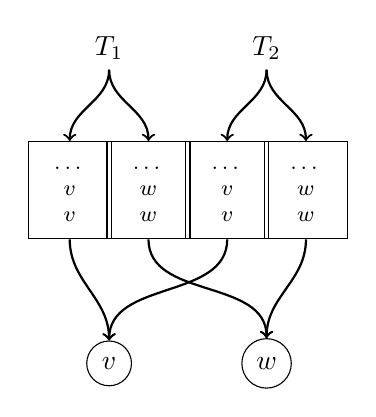
\begin{tikzpicture}
      \node (t1) at (-1,0) {$T_1$};
      \node (t2) at (1,0)  {$T_2$};
      \node (v) [draw,shape=circle] at (-1,-4) {$v$};
      \node (w) [draw,shape=circle] at (1,-4)  {$w$};

      \node (bt1v) [draw] at (-1.5,-1.8) {\footnotesize\begin{tabular}{c} \ldots \\\midrule $v$ \\\midrule $v$ \end{tabular}};
      \node (bt1w) [draw] at (-0.5,-1.8) {\footnotesize\begin{tabular}{c} \ldots \\\midrule $w$ \\\midrule $w$ \end{tabular}};
      \node (bt2v) [draw] at (0.5,-1.8) {\footnotesize\begin{tabular}{c} \ldots \\\midrule $v$ \\\midrule $v$ \end{tabular}};
      \node (bt2w) [draw] at (1.5,-1.8) {\footnotesize\begin{tabular}{c} \ldots \\\midrule $w$ \\\midrule $w$ \end{tabular}};

      \draw [->, thick] (t1) to [out=270,in=90] (bt1v);
      \draw [->, thick] (t1) to [out=270,in=90] (bt1w);
      \draw [->, thick] (t2) to [out=270,in=90] (bt2v);
      \draw [->, thick] (t2) to [out=270,in=90] (bt2w);

      \draw [->, thick] (bt1v.south) to [out=270,in=90] (v);
      \draw [->, thick] (bt1w.south) to [out=270,in=90] (w);
      \draw [->, thick] (bt2v.south) to [out=270,in=90] (v);
      \draw [->, thick] (bt2w.south) to [out=270,in=90] (w);
    \end{tikzpicture}
    \caption{Partial Store Order}
  \end{subfigure}
  \caption{Example of write buffering for two threads and two \texttt{IORef}s.}
  \label{fig:wb}
\end{figure}

We divide operations into three categories: \emph{synchronised}
operations impose a \emph{memory barrier}, committing all writes;
\emph{partially synchronised} operations commit one or more writes to
the same \verb|IORef|; and \emph{unsynchronised} operations never cause
a commit.

\paragraph{Phantom threads}
In a sequentially consistent memory model, the set of runnable threads
is exactly the set of threads created by forking which are not
blocked.  Under our model of relaxed memory, however, this is not the
case.  For each write buffer, we introduce one \emph{phantom thread}.
When scheduled, a phantom thread commits the oldest write in its
corresponding buffer.

This may seem like an odd approach: why create new threads to model
relaxed memory?  By using phantom threads, relaxed memory
nondeterminism becomes just another aspect of scheduling
nondeterminism.  We take this approach from \cite{zhang2015}.

\section{Operational Semantics}
\label{sec:dejafu-semantics}

Fundamental to how \dejafu{} works is an operational semantics for
Haskell concurrency, in the form of a step function on primitive
actions.  Given the current state, which we call the context, the
identifier of the chosen thread, and its primitive action, we either
indicate a failure condition, or produce a new context; in both cases
we return a log of what happened, to put into the execution trace
returned to the user.  The STM primitive actions also have an
operational semantics.  As transactions are atomic, we only care about
the big-step behaviour.  This simplifies some aspects of their
implementation.

\paragraph{The heap}
We implement \verb|IORef|s, \verb|MVar|s, and \verb|TVar|s with mutable
references.  We do not use a pure model of the heap, as we found the
additional indirection to both increase allocation, and to reduce the
efficacy of garbage collection.  By using references directly, when
all copies of a reference fall out of scope, the referenced value can
be garbage collected.  If we model references as keys into a
heterogeneous map, then such data can never be freed, as we cannot
tell when it is safe to delete a key.

This means that executing our step function has effects, and in
general contexts cannot be re-used.  For general concurrency, this is
not a limitation in practice because we never want to re-use contexts.
However, for STM, we do have to compute an action to undo effects,
which is applied if a transaction fails.

To simplify the presentation of rules, we use a pure heap model in
this section.

\subsection{Semantics of Concurrency}

We express our concurrency semantics as transition rules for a context
tuple $\langle\texttt{C}, \texttt{B}, \texttt{H}, \texttt{T}\rangle$:

\begin{itemize}
\item \verb|C| is the number of capabilities.
\item \verb|B| is the relaxed-memory buffer state.
\item \verb|H| is the heap, a heterogeneous map from identifiers to
  Haskell values.
\item \verb|T| is a mapping from thread identifiers to threads.
\end{itemize}

We express threads as records supporting both access and update.  For
a thread \verb|t|:

\begin{itemize}
\item \verb|t.K| is its current continuation.
\item \verb|t.I| is the set of identifiers it is blocked on.
\item \verb|t.E| is its exception handler stack.
\item \verb|t.M| is its exception masking state.
\end{itemize}

We write $\texttt{H}_{[\texttt{id} \mapsto \texttt{v}]}$ to denote a
new heap which maps \texttt{id} to the Haskell value \texttt{v}, and
$\texttt{T}_{[\texttt{id}.\texttt{K} \mapsto \texttt{c}]}$ to denote a
new thread map where the continuation of thread \texttt{id} is now
\texttt{c}, and similarly for other fields.

There are two global bindings which are in scope for every rule:
(1)~\verb|memtype|, the memory model for relaxed memory operations,
which is \verb|SequentialConsistency|, \verb|TotalStoreOrder|, or
\verb|PartialStoreOrder|; and (2)~\verb|tid|, the identifier of the
currently executing thread.

For some rules we include side-conditions or local definitions.  We
use Haskell syntax for these.

\paragraph{Simplifications and omissions}
The semantic rules we present are for the small-step behaviour.  They
are tied together by a scheduling loop which we do not present here.
This scheduling loop picks a thread to step, steps it, and continues
until every thread is blocked or the main thread terminates.

In addition to modelling the heap as part of the context, we make some
other changes for presentation purposes.  We omit building the
execution trace; we omit the definitions of helper functions, but
explain them when first used; and we omit the semantic rules for
\verb|ASub| and \verb|AStopSub|.  The \verb|ASub| and \verb|AStopSub|
actions implement a \dejafu{}-specific utility function, and are not
essential to the concurrency model.

\begin{figure}
\centering
\begin{tabular}{r@{\hspace{0.5em}}l}
$\langle\texttt{C}, \texttt{B}, \texttt{H}, \texttt{T}\rangle
\xrightarrow{\texttt{\small AFork act c}}$&
$\langle\texttt{C}, \texttt{B}, \texttt{H}, \texttt{T}_{[\texttt{id} \mapsto \texttt{new};~\texttt{tid}.\texttt{K} \mapsto \texttt{c id}]}\rangle$\\
\multicolumn{2}{l}{where \texttt{id} is fresh}\\
\multicolumn{2}{l}{\hphantom{where }$\texttt{m0} = \texttt{T}_{[\texttt{tid}.\texttt{M}]}$}\\
\multicolumn{2}{l}{\hphantom{where }$\texttt{reset m'} = \texttt{\textbackslash k -> AResetMask m' (k ())}$}\\
\multicolumn{2}{l}{\hphantom{where }$\texttt{umask mb} = \texttt{reset Unmasked >> mb >> \textbackslash b -> reset m0 >> pure b}$}\\
\multicolumn{2}{l}{\hphantom{where }$\texttt{new} = \texttt{Thread \{ K = act umask, I = }\varnothing\texttt{, E = [], M = m0 \}}$}\\
& \\
$\langle\texttt{C}, \texttt{B}, \texttt{H}, \texttt{T}\rangle
\xrightarrow{\texttt{\small ALift n}}$&
$\langle\texttt{C}, \texttt{B}, \texttt{H}, \texttt{T}_{[\texttt{tid}.\texttt{K} \mapsto \texttt{c ()}]}\rangle$\\
\multicolumn{2}{l}{where \texttt{c} is the result of executing the Haskell action \texttt{n}}\\
& \\
$\langle\texttt{C}, \texttt{B}, \texttt{H}, \texttt{T}\rangle
\xrightarrow{\texttt{\small AGetNumCapabilities c}}$&
$\langle\texttt{C}, \texttt{B}, \texttt{H}, \texttt{T}_{[\texttt{tid}.\texttt{K} \mapsto \texttt{c C}]}\rangle$\\
$\langle\texttt{C}, \texttt{B}, \texttt{H}, \texttt{T}\rangle
\xrightarrow{\texttt{\small ASetNumCapabilities i c}}$&
$\langle\texttt{i}, \texttt{B}, \texttt{H}, \texttt{T}_{[\texttt{tid}.\texttt{K} \mapsto \texttt{c ()}]}\rangle$\\
$\langle\texttt{C}, \texttt{B}, \texttt{H}, \texttt{T}\rangle
\xrightarrow{\texttt{\small AMyTId c}}$&
$\langle\texttt{C}, \texttt{B}, \texttt{H}, \texttt{T}_{[\texttt{tid}.\texttt{K} \mapsto \texttt{c tid}]}\rangle$\\
$\langle\texttt{C}, \texttt{B}, \texttt{H}, \texttt{T}\rangle
\xrightarrow{\texttt{\small AYield c}}$&
$\langle\texttt{C}, \texttt{B}, \texttt{H}, \texttt{T}_{[\texttt{tid}.\texttt{K} \mapsto \texttt{c ()}]}\rangle$\\
$\langle\texttt{C}, \texttt{B}, \texttt{H}, \texttt{T}\rangle
\xrightarrow{\texttt{\small ADelay c}}$&
$\langle\texttt{C}, \texttt{B}, \texttt{H}, \texttt{T}_{[\texttt{tid}.\texttt{K} \mapsto \texttt{c ()}]}\rangle$\\
$\langle\texttt{C}, \texttt{B}, \texttt{H}, \texttt{T}\rangle
\xrightarrow{\texttt{\small AReturn c}}$&
$\langle\texttt{C}, \texttt{B}, \texttt{H}, \texttt{T}_{[\texttt{tid}.\texttt{K} \mapsto \texttt{c ()}]}\rangle$\\
$\langle\texttt{C}, \texttt{B}, \texttt{H}, \texttt{T}\rangle
\xrightarrow{\texttt{\small AStop}}$&
$\langle\texttt{C}, \texttt{B}, \texttt{H}, \texttt{T}_{[\texttt{tid} \mapsto \varnothing]}\rangle$
\end{tabular}
\caption{Transition semantics of basic multithreading actions.}\label{fig:sem_multithreading}
\end{figure}

\paragraph{Rules for basic multithreading}
\Cref{fig:sem_multithreading} shows the semantics for the basic
multithreading operations.  The rule for \verb|AFork| implements
\verb|forkWithUnmask|, so it constructs a function to run an action
umasked.  The \verb|fork| function is a special case of
\verb|forkWithUnmask| which ignores this argument.  There is no
separate action for \verb|forkOn|, as we do not model which capability
a thread is executing on.  We use ``\verb|id| is fresh'' to mean that
\verb|id| is a new, globally unique, identifier.  We use
$\texttt{T}_{[\texttt{tid}\mapsto\varnothing]}$ to mean that the
thread is deleted.

The \verb|ALift| action is special, as it causes a Haskell-level
effect to occur.  It produces a continuation by executing some
\verb|IO| action.

\paragraph{Rules for \texttt{IORef} operations}
\Cref{fig:sem_ioref} shows the semantics for the \verb|IORef|
operations.  We represent a \verb|IORef| as reference to a pair of a
number of commits and a latest value.

We use $\texttt{H} \oplus \texttt{B}$ to mean a new heap with all
writes from each buffer committed, in order.  This is a memory
barrier.  The order in which buffers are committed is deterministic,
but arbitrary.  So in general, $\oplus$ will cause the writes of one
thread to `win'.  The DPOR machinery imposes a dependency between such
barrier actions and \verb|ACommit| actions, so in practice we do
explore different orderings of commits.  We use
$\texttt{H} \oplus \texttt{B}_{[\texttt{tid}]}$ to mean that only the
buffered writes from thread \verb|tid| are committed.

We use $\texttt{B} + \texttt{(tid, id, a)}$ to mean a new buffer
state, with a write of value \verb|a| to \verb|IORef| \verb|id| by
thread \verb|tid| buffered.  We use $\texttt{B} - \texttt{(tid, id)}$
to mean removing the oldest buffered write to \verb|IORef| \verb|id| by
thread \verb|tid| from the buffer.

The \verb|ACommit| action has no continuation.  The phantom threads
which we introduce to perform commits are created before the scheduler
is invoked, and deleted after each action.  There is always one
phantom thread for each nonempty buffer, and no more.

\paragraph{Rules for \texttt{MVar} operations}
\Cref{fig:sem_mvar} shows the semantics for the \verb|MVar|
operations.  We represent an \verb|MVar| as a reference to a
\verb|Maybe| value.  These operations enforce a write barrier, and
some of them may cause the thread to block.  We model a thread
blocking by storing the identifiers it is blocked on, and leaving its
continuation untouched.  The scheduler loop will not choose the thread
again until it is unblocked.  We use
$\texttt{T} \Uparrow \texttt{ids}$ to mean that we unblock all threads
blocked on any of the given identifiers.

\paragraph{Rules for exceptions and masking}
\Cref{fig:sem_exc} shows the semantics for the exception and masking
operations.  The \verb|raise| function pops from a thread's exception
handler stack until it finds a handler for the given exception.  The
\verb|interruptible| function checks if the given thread can be
interrupted with an exception.

The \verb|AThrowTo| action can cause a thread to block, but there are
no rules here which would unblock the thread: this is handled in the
scheduler loop.  Many of the rules affect whether a thread can receive
an asynchronous exception, so we handle it in one place.

The \verb|AMasking| action is similar to \verb|AFork|: it runs an
action after passing an argument to change the masking state.  Only,
\verb|AMasking| runs the action in the current thread.

\begin{figure}
\centering
\begin{tabular}{r@{\hspace{0.5em}}l}
$\langle\texttt{C}, \texttt{B}, \texttt{H}, \texttt{T}\rangle
\xrightarrow{\texttt{\small ANewIORef a c}}$&
$\langle\texttt{C}, \texttt{B}, \texttt{H}_{[\texttt{id} \mapsto \texttt{(0, a)}]}, \texttt{T}_{[\texttt{tid}.\texttt{K} \mapsto \texttt{c id}]}\rangle$ \\
\multicolumn{2}{l}{where \texttt{id} is fresh}\\
& \\
$\langle\texttt{C}, \texttt{B}, \texttt{H}, \texttt{T}\rangle
\xrightarrow{\texttt{\small AReadIORef id c}}$&
$\langle\texttt{C}, \texttt{B}, \texttt{H}, \texttt{T}_{[\texttt{tid}.\texttt{K} \mapsto \texttt{c x}]}\rangle$ \\
\multicolumn{2}{l}{where $(\texttt{H} \oplus \texttt{B}_{[\texttt{tid}]})_{[\texttt{id}]} = \texttt{(\_, x)}$}\\
& \\
$\langle\texttt{C}, \texttt{B}, \texttt{H}, \texttt{T}\rangle
\xrightarrow{\texttt{\small AReadIORefCAS id c}}$&
$\langle\texttt{C}, \texttt{B}, \texttt{H}, \texttt{T}_{[\texttt{tid}.\texttt{K} \mapsto \texttt{c (Ticket id n x)}]}\rangle$ \\
\multicolumn{2}{l}{where $(\texttt{H} \oplus \texttt{B}_{[\texttt{tid}]})_{[\texttt{id}]} = \texttt{(n, x)}$}\\
& \\
$\langle\texttt{C}, \texttt{B}, \texttt{H}, \texttt{T}\rangle
\xrightarrow{\texttt{\small AWriteIORef id a c}}$&
$\langle\texttt{C}, \texttt{B}, \texttt{H}_{[\texttt{id} \mapsto \texttt{(0, a)}]}, \texttt{T}_{[\texttt{tid}.\texttt{K} \mapsto \texttt{c ()}]}\rangle$ \\
\multicolumn{2}{l}{if $\texttt{memtype} = \texttt{SequentialConsistency}$}\\
& \\
$\langle\texttt{C}, \texttt{B}, \texttt{H}, \texttt{T}\rangle
\xrightarrow{\texttt{\small AWriteIORef id a c}}$&
$\langle\texttt{C}, \texttt{B} + \texttt{(tid, id, a)}, \texttt{H}, \texttt{T}_{[\texttt{tid}.\texttt{K} \mapsto \texttt{c ()}]}\rangle$ \\
\multicolumn{2}{l}{if $\texttt{memtype} \neq \texttt{SequentialConsistency}$}\\
& \\
$\langle\texttt{C}, \texttt{B}, \texttt{H}, \texttt{T}\rangle
\xrightarrow{\texttt{\small AModIORef id f c}}$&
$\langle\texttt{C}, \varnothing, (\texttt{H} \oplus \texttt{B})_{[\texttt{id} \mapsto \texttt{(n+1, f a)}]}, \texttt{T}_{[\texttt{tid}.\texttt{K} \mapsto \texttt{c ()}]}\rangle$ \\
\multicolumn{2}{l}{where $\texttt{H} \oplus \texttt{B}_{[\texttt{tid}]} = \texttt{(n, a)}$}\\
& \\
$\langle\texttt{C}, \texttt{B}, \texttt{H}, \texttt{T}\rangle
\xrightarrow{\texttt{\small AModIORefCAS id f c}}$&
$\langle\texttt{C}, \varnothing, (\texttt{H} \oplus \texttt{B})_{[\texttt{id} \mapsto \texttt{(n+1, f a)}]}, \texttt{T}_{[\texttt{tid}.\texttt{K} \mapsto \texttt{c ()}]}\rangle$ \\
\multicolumn{2}{l}{where $(\texttt{H} \oplus \texttt{B})_{[\texttt{id}]} = \texttt{(n, a)}$}\\
& \\
\multicolumn{2}{l}{$\langle\texttt{C}, \texttt{B}, \texttt{H}, \texttt{T}\rangle
\xrightarrow{\texttt{\small ACasIORef id (Ticket id n \_) a c}}$}\\
\multicolumn{2}{l}{\hfill $\langle\texttt{C}, \varnothing, (\texttt{H} \oplus \texttt{B})_{[\texttt{id} \mapsto \texttt{(n+1, a)}]}, \texttt{T}_{[\texttt{tid}.\texttt{K} \mapsto \texttt{c (True, Ticket id (n+1) a)}]}\rangle$}\\
\multicolumn{2}{l}{if $\texttt{n} = \texttt{n0}$}\\
\multicolumn{2}{l}{where $(\texttt{H} \oplus \texttt{B})_{[\texttt{id}]} = \texttt{(n0, \_)}$}\\
& \\
\multicolumn{2}{l}{$\langle\texttt{C}, \texttt{B}, \texttt{H}, \texttt{T}\rangle
\xrightarrow{\texttt{\small ACasIORef id (Ticket id n \_) \_ c}}$}\\
\multicolumn{2}{l}{\hfill $\langle\texttt{C}, \varnothing, \texttt{H} \oplus \texttt{B}, \texttt{T}_{[\texttt{tid}.\texttt{K} \mapsto \texttt{c (False, Ticket id n0 a0)}]}\rangle$}\\
\multicolumn{2}{l}{if $\texttt{n} \neq \texttt{n0}$}\\
\multicolumn{2}{l}{where $(\texttt{H} \oplus \texttt{B})_{[\texttt{id}]} = \texttt{(n0, a0)}$}\\
& \\
$\langle\texttt{C}, \texttt{B}, \texttt{H}, \texttt{T}\rangle
\xrightarrow{\texttt{\small ACommit idT idC}}$&
$\langle\texttt{C}, \texttt{B'}, \texttt{H}_{[\texttt{id} \mapsto \texttt{(n+1, a)}]}, \texttt{T}\rangle$\\
\multicolumn{2}{l}{where $\texttt{H}_{[\texttt{id}]} = \texttt{(n, \_)}$}\\
\multicolumn{2}{l}{\hphantom{where }$\texttt{B} - \texttt{(tid, id)} = \texttt{(B', a')}$}
\end{tabular}
\caption{Transition semantics of \texttt{IORef} actions.}\label{fig:sem_ioref}
\end{figure}

\begin{figure}
\centering
\begin{tabular}{r@{\hspace{0.5em}}l}
$\langle\texttt{C}, \texttt{B}, \texttt{H}, \texttt{T}\rangle
\xrightarrow{\texttt{\small ANewMVar c}}$&
$\langle\texttt{C}, \texttt{B}, \texttt{H}_{[\texttt{id} \mapsto \texttt{Nothing}]}, \texttt{T}_{[\texttt{tid}.\texttt{K} \mapsto \texttt{c id}]}\rangle$ \\
\multicolumn{2}{l}{where \texttt{id} is fresh}\\
& \\
$\langle\texttt{C}, \texttt{B}, \texttt{H}, \texttt{T}\rangle
\xrightarrow{\texttt{\small APutMVar id \_{}}}$&
$\langle\texttt{C}, \varnothing, \texttt{H} \oplus \texttt{B}, \texttt{T}_{[\texttt{tid}.\texttt{I} \mapsto \{\texttt{id}\}]}\rangle$\\
\multicolumn{2}{l}{if $\texttt{H}_{[\texttt{id}]} = \texttt{Just \_}$}\\
& \\
$\langle\texttt{C}, \texttt{B}, \texttt{H}, \texttt{T}\rangle
\xrightarrow{\texttt{\small APutMVar id a c}}$&
$\langle\texttt{C}, \varnothing, \texttt{H}_{[\texttt{id} \mapsto \texttt{Just a}]} \oplus \texttt{B}, \texttt{T}_{[\texttt{tid}.\texttt{K} \mapsto \texttt{c ()}]} \Uparrow \{\texttt{id}\}\rangle$\\
\multicolumn{2}{l}{if $\texttt{H}_{[\texttt{id}]} = \texttt{Nothing}$}\\
& \\
$\langle\texttt{C}, \texttt{B}, \texttt{H}, \texttt{T}\rangle
\xrightarrow{\texttt{\small ATakeMVar id c}}$&
$\langle\texttt{C}, \varnothing, \texttt{H}_{[\texttt{id} \mapsto \texttt{Nothing}]} \oplus \texttt{B}, \texttt{T}_{[\texttt{tid}.\texttt{K} \mapsto \texttt{c x}]} \Uparrow \{\texttt{id}\}\rangle$\\
\multicolumn{2}{l}{if $\texttt{H}_{[\texttt{id}]} = \texttt{Just x}$}\\
& \\
$\langle\texttt{C}, \texttt{B}, \texttt{H}, \texttt{T}\rangle
\xrightarrow{\texttt{\small ATakeMVar id \_}}$&
$\langle\texttt{C}, \varnothing, \texttt{H} \oplus \texttt{B}, \texttt{T}_{[\texttt{tid}.\texttt{I} \mapsto \{\texttt{id}\}]}\rangle$\\
\multicolumn{2}{l}{if $\texttt{H}_{[\texttt{id}]} = \texttt{Nothing}$} \\
& \\
$\langle\texttt{C}, \texttt{B}, \texttt{H}, \texttt{T}\rangle
\xrightarrow{\texttt{\small AReadMVar id c}}$&
$\langle\texttt{C}, \varnothing, \texttt{H} \oplus \texttt{B}, \texttt{T}_{[\texttt{tid}.\texttt{K} \mapsto \texttt{c x}]}\rangle$\\
\multicolumn{2}{l}{if $\texttt{H}_{[\texttt{id}]} = \texttt{Just x}$}\\
& \\
$\langle\texttt{C}, \texttt{B}, \texttt{H}, \texttt{T}\rangle
\xrightarrow{\texttt{\small AReadMVar id \_}}$&
$\langle\texttt{C}, \varnothing, \texttt{H} \oplus \texttt{B}, \texttt{T}_{[\texttt{tid}.\texttt{I} \mapsto \{\texttt{id}\}]}\rangle$\\
\multicolumn{2}{l}{if $\texttt{H}_{[\texttt{id}]} = \texttt{Nothing}$}\\
& \\
$\langle\texttt{C}, \texttt{B}, \texttt{H}, \texttt{T}\rangle
\xrightarrow{\texttt{\small ATryPutMVar id c}}$&
$\langle\texttt{C}, \varnothing, \texttt{H} \oplus \texttt{B}, \texttt{T}_{[\texttt{tid}.\texttt{K} \mapsto \texttt{c False}]}\rangle$\\
\multicolumn{2}{l}{if $\texttt{H}_{[\texttt{id}]} = \texttt{Just \_}$}\\
& \\
$\langle\texttt{C}, \texttt{B}, \texttt{H}, \texttt{T}\rangle
\xrightarrow{\texttt{\small ATryPutMVar id a c}}$&
$\langle\texttt{C}, \varnothing, \texttt{H}_{[\texttt{id} \mapsto \texttt{Just a}]} \oplus \texttt{B}, \texttt{T}_{[\texttt{tid}.\texttt{K} \mapsto \texttt{c True}]} \Uparrow \{\texttt{id}\}\rangle$\\
\multicolumn{2}{l}{if $\texttt{H}_{[\texttt{id}]} = \texttt{Nothing}$}\\
& \\
$\langle\texttt{C}, \texttt{B}, \texttt{H}, \texttt{T}\rangle
\xrightarrow{\texttt{\small ATryTakeMVar id c}}$& \\
\multicolumn{2}{l}{\hfill $\langle\texttt{C}, \varnothing, \texttt{H}_{[\texttt{id} \mapsto \texttt{Nothing}]} \oplus \texttt{B}, \texttt{T}_{[\texttt{tid}.\texttt{K} \mapsto \texttt{c (Just x)}]} \Uparrow \{\texttt{id}\}\rangle$}\\
\multicolumn{2}{l}{if $\texttt{H}_{[\texttt{id}]} = \texttt{Just x}$}\\
& \\
$\langle\texttt{C}, \texttt{B}, \texttt{H}, \texttt{T}\rangle
\xrightarrow{\texttt{\small ATryTakeMVar id c}}$&
$\langle\texttt{C}, \varnothing, \texttt{H} \oplus \texttt{B}, \texttt{T}_{[\texttt{tid}.\texttt{K} \mapsto \texttt{c Nothing}]}\rangle$\\
\multicolumn{2}{l}{if $\texttt{H}_{[\texttt{id}]} = \texttt{Nothing}$} \\
& \\
$\langle\texttt{C}, \texttt{B}, \texttt{H}, \texttt{T}\rangle
\xrightarrow{\texttt{\small ATryReadMVar id c}}$&
$\langle\texttt{C}, \varnothing, \texttt{H} \oplus \texttt{B}, \texttt{T}_{[\texttt{tid}.\texttt{K} \mapsto \texttt{c H}_{[\texttt{id}]}]}\rangle$
\end{tabular}
\caption{Transition semantics of \texttt{MVar} actions.}\label{fig:sem_mvar}
\end{figure}

\begin{figure}
\centering
\begin{tabular}{r@{\hspace{0.5em}}l}
$\langle\texttt{C}, \texttt{B}, \texttt{H}, \texttt{T}\rangle
\xrightarrow{\texttt{\small AThrow e}}$&
$\langle\texttt{C}, \texttt{B}, \texttt{H}, \texttt{T}_{[\texttt{tid}.\texttt{I} \mapsto \varnothing;~\texttt{tid}.\texttt{E} \mapsto \texttt{hs};~\texttt{tid}.\texttt{K} \mapsto \texttt{h e}]}\rangle$ \\
\multicolumn{2}{l}{if $\texttt{raise T}_{[\texttt{tid}]}~\texttt{e} = \texttt{h:hs}$}\\
& \\
$\langle\texttt{C}, \texttt{B}, \texttt{H}, \texttt{T}\rangle
\xrightarrow{\texttt{\small AThrow e}}$&
$\langle\texttt{C}, \texttt{B}, \texttt{H}, \texttt{T}_{[\texttt{tid} \mapsto \varnothing]}\rangle$ \\
\multicolumn{2}{l}{if $\texttt{raise T}_{[\texttt{tid}]}~\texttt{e} = \texttt{[]}$}\\
& \\
$\langle\texttt{C}, \texttt{B}, \texttt{H}, \texttt{T}\rangle
\xrightarrow{\texttt{\small AThrowTo id e c}}$&\\
\multicolumn{2}{r}{$\langle\texttt{C}, \varnothing, \texttt{H} \oplus \texttt{B}, \texttt{T}_{[\texttt{tid}.\texttt{K} \mapsto \texttt{c ()};~\texttt{id}.\texttt{I} \mapsto \varnothing;~\texttt{id}.\texttt{E} \mapsto \texttt{hs};~\texttt{id}.\texttt{K} \mapsto \texttt{h e}]}\rangle$} \\
\multicolumn{2}{l}{if $\texttt{interruptible T}_{[\texttt{id}]}$}\\
\multicolumn{2}{l}{\hphantom{if }$\texttt{raise T}_{[\texttt{id}]}~\texttt{e} = \texttt{h:hs}$}\\
& \\
$\langle\texttt{C}, \texttt{B}, \texttt{H}, \texttt{T}\rangle
\xrightarrow{\texttt{\small AThrowTo id e c}}$&
$\langle\texttt{C}, \varnothing, \texttt{H} \oplus \texttt{B}, \texttt{T}_{[\texttt{tid}.\texttt{K} \mapsto \texttt{c ()};~\texttt{id} \mapsto \varnothing]}\rangle$ \\
\multicolumn{2}{l}{if $\texttt{interruptible T}_{[\texttt{id}]}$}\\
\multicolumn{2}{l}{\hphantom{if }$\texttt{raise T}_{[\texttt{id}]}~\texttt{e} = \texttt{[]}$}\\
& \\
$\langle\texttt{C}, \texttt{B}, \texttt{H}, \texttt{T}\rangle
\xrightarrow{\texttt{\small AThrowTo id e c}}$&
$\langle\texttt{C}, \varnothing, \texttt{H} \oplus \texttt{B}, \texttt{T}_{[\texttt{tid}.\texttt{I} \mapsto \{\texttt{id}\}]}\rangle$ \\
\multicolumn{2}{l}{if $\lnot~ \texttt{interruptible T}_{[\texttt{id}]}$}\\
& \\
$\langle\texttt{C}, \texttt{B}, \texttt{H}, \texttt{T}\rangle
\xrightarrow{\texttt{\small ACatching i inner c}}$&\\
\multicolumn{2}{r}{$\langle\texttt{C}, \texttt{B}, \texttt{H}, \texttt{T}_{[\texttt{tid}.\texttt{K} \mapsto \texttt{inner (APopCatching . c)};~\texttt{tid}.\texttt{I} \mapsto \texttt{h:hs}]\rangle}$} \\
\multicolumn{2}{l}{where $\texttt{T}_{[\texttt{tid}.\texttt{E}]} = \texttt{hs}$}\\
& \\
$\langle\texttt{C}, \texttt{B}, \texttt{H}, \texttt{T}\rangle
\xrightarrow{\texttt{\small APopCatching c}}$&
$\langle\texttt{C}, \texttt{B}, \texttt{H}, \texttt{T}_{[\texttt{tid}.\texttt{K} \mapsto \texttt{c ()};~\texttt{tid}.\texttt{I} \mapsto \texttt{hs}]\rangle}$ \\
\multicolumn{2}{l}{where $\texttt{T}_{[\texttt{tid}.\texttt{E}]} = \texttt{\_:hs}$}\\
& \\
$\langle\texttt{C}, \texttt{B}, \texttt{H}, \texttt{T}\rangle
\xrightarrow{\texttt{\small AMasking m act c}}$&\\
\multicolumn{2}{r}{$\langle\texttt{C}, \texttt{B}, \texttt{H}, \texttt{T}_{[\texttt{tid}.\texttt{K} \mapsto \texttt{act umask (AResetMask m0 . c)};~\texttt{tid}.\texttt{M} \mapsto \texttt{m}]}\rangle$} \\
\multicolumn{2}{l}{where $\texttt{m0} = \texttt{T}_{[\texttt{tid}.\texttt{M}]}$}\\
\multicolumn{2}{l}{\hphantom{where }$\texttt{reset m'} = \texttt{\textbackslash k -> AResetMask m' (k ())}$}\\
\multicolumn{2}{l}{\hphantom{where }$\texttt{umask mb} = \texttt{reset m0 >> mb >> \textbackslash b -> reset m >> pure b}$}\\
& \\
$\langle\texttt{C}, \texttt{B}, \texttt{H}, \texttt{T}\rangle
\xrightarrow{\texttt{\small AResetMask m c}}$&
$\langle\texttt{C}, \texttt{B}, \texttt{H}, \texttt{T}_{[\texttt{tid}.\texttt{K} \mapsto \texttt{c ()};~\texttt{tid}.\texttt{M} \mapsto \texttt{m}]}\rangle$
\end{tabular}
\caption{Transition semantics of exception actions.}\label{fig:sem_exc}
\end{figure}

\FloatBarrier
\subsection{Semantics of Software Transactional Memory}

We express our STM semantics similarly, as transition rules for a
context tuple
$\langle\texttt{H}, \texttt{K}, \texttt{R}, \texttt{W}\rangle$:

\begin{itemize}
\item \verb|H|, the heap.
\item \verb|K|, the current continuation.
\item \verb|R|, the set of \verb|TVar|s which have been read from.
\item \verb|W|, the set of \verb|TVar|s which have been written to.
\end{itemize}

From the point of view of a transaction there is only one thread,
which is the one executing the transaction.  So our context does not
contain a thread map, as with concurrency, but just the single
continuation of interest.  We also track which \verb|TVar|s have been
read from or written to, which are used to handle blocking of aborted
transactions, and in the DPOR implementation to determine dependency
between transactions.

\begin{figure}[h]
\centering
\begin{tabular}{r@{\hspace{0.5em}}l}
$\langle\texttt{C}, \texttt{B}, \texttt{H}, \texttt{T}\rangle
\xrightarrow{\texttt{\small AAtom stm c}}$&
$\langle\texttt{C}, \varnothing, \texttt{H'} \oplus \texttt{B}, \texttt{T}_{[\texttt{tid}.\texttt{K} \mapsto \texttt{c a}]} \Uparrow \texttt{W}\rangle$\\
\multicolumn{2}{l}{if $\texttt{runSTM H stm} = \texttt{(Success a H', \_, W)}$} \\
& \\
$\langle\texttt{C}, \texttt{B}, \texttt{H}, \texttt{T}\rangle
\xrightarrow{\texttt{\small AAtom stm \_}}$&
$\langle\texttt{C}, \varnothing, \texttt{H} \oplus \texttt{B}, \texttt{T}_{[\texttt{tid}.\texttt{I} \mapsto \texttt{R}]}\rangle$\\
\multicolumn{2}{l}{if $\texttt{runSTM H stm} = \texttt{(Aborted, R, \_)}$} \\
& \\
$\langle\texttt{C}, \texttt{B}, \texttt{H}, \texttt{T}\rangle
\xrightarrow{\texttt{\small AAtom stm \_}}$&
$\langle\texttt{C}, \varnothing, \texttt{H} \oplus \texttt{B}, \texttt{T}_{[\texttt{tid}.\texttt{K} \mapsto \texttt{AThrow e}]}\rangle$\\
\multicolumn{2}{l}{if $\texttt{runSTM H stm} = \texttt{(Exception e, \_, \_)}$}
\end{tabular}
\caption{Transition semantics for \texttt{AAtom}.}\label{fig:sem_aatom}
\end{figure}

\paragraph{Rules for executing transactions}
\Cref{fig:sem_aatom} shows the semantics for \verb|AAtom|, the bridge
between the concurrency and the STM semantics, where the \verb|runSTM|
function runs a transaction to completion.  There are three possible
results: (1)~the transaction succeeded, which gives the final value
and the new heap; (2)~the transaction was aborted; and (3)~an uncaught
exception was raised, which gives the exception.  Each case also
returns the \verb|TVar|s read from and written to.  Executing a
transaction enforces a memory barrier, regardless of the result.

As we have modelled the heap as a pure heterogeneous map in our
semantics, we do not need to explicitly undo the effects of an
unsuccessful transaction.  We simply discard the updated heap.  In the
real implementation, we construct and apply an action to undo the
effects of a transaction.

\paragraph{Rules for basic STM actions}
\Cref{fig:sem_stm1} shows the basic STM actions.  The \verb|SRetry|,
\verb|SThrow|, and \verb|SStop| actions all end the transaction, but
do not contain a continuation.  They are recognised by the
\verb|runSTM| function, and cause it to return.

\paragraph{Rules for catching \texttt{SRetry}}
\Cref{fig:sem_stm2} shows the semantics for the \verb|SOrElse| action,
which catches \verb|SRetry|.  The three cases where the first
transaction aborts reveal a subtle detail: when the first transaction
aborts, the \verb|TVar|s it has read must still be included in the set
that the transaction as a whole read from.  It may not have called
\verb|SRetry| if those \verb|TVar|s had a different value.  If the
transaction as a whole is aborted, throwing away those \verb|TVar|
identifiers could result in the thread not being unblocked where it
should
be\footnote{\url{https://github.com/barrucadu/dejafu/issues/55}}.

\paragraph{Rules for catching \texttt{SThrow}}
\Cref{fig:sem_stm3} shows the semantics for the \verb|SCatch| action,
which catches \verb|SThrow| if the exception is of the appropriate
type.  The \verb|handles| function checks if the handler can handle
that exception type.  This is similar to \verb|raise| for the
concurrency semantic rules, but it only looks at one exception
handler, rather than a stack of them.

\paragraph{Big-step semantics}
Both \verb|SOrElse| and \verb|SCatch| look more like what you would
expect in a big-step semantics than a small-step semantics, as they
evaluate entire transactions.  We use this style because transactions
are atomic, and it simplifies the implementation.

\begin{figure}
\centering
\begin{tabular}{r@{\hspace{0.5em}}l}
$\langle\texttt{H}, \_, \texttt{R}, \texttt{W}\rangle
\xrightarrow{\texttt{\small SNew a c}}$&
$\langle\texttt{H}_{[\texttt{id} \mapsto \texttt{a}]}, \texttt{c id}, \texttt{R}, \texttt{W}\rangle$\\
\multicolumn{2}{l}{where \texttt{id} is fresh}\\
& \\
$\langle\texttt{H}, \_, \texttt{R}, \texttt{W}\rangle
\xrightarrow{\texttt{\small SRead id c}}$&
$\langle\texttt{H}, \texttt{c H}_{[\texttt{id}]}, \{\texttt{id}\} \cup \texttt{R}, \texttt{W}\rangle$\\
$\langle\texttt{H}, \_, \texttt{R}, \texttt{W}\rangle
\xrightarrow{\texttt{\small SWrite id a c}}$&
$\langle\texttt{H}_{[\texttt{id} \mapsto \texttt{a}]}, \texttt{c ()}, \texttt{R}, \{\texttt{id}\} \cup \texttt{W}\rangle$\\
$\langle\texttt{H}, \texttt{K}, \texttt{R}, \texttt{W}\rangle
\xrightarrow{\texttt{\small SRetry}}$&
$\langle\texttt{H}, \texttt{K}, \texttt{R}, \texttt{W}\rangle$\\
$\langle\texttt{H}, \texttt{K}, \texttt{R}, \texttt{W}\rangle
\xrightarrow{\texttt{\small SThrow \_}}$&
$\langle\texttt{H}, \texttt{K}, \texttt{R}, \texttt{W}\rangle$\\
$\langle\texttt{H}, \texttt{K}, \texttt{R}, \texttt{W}\rangle
\xrightarrow{\texttt{\small SStop}}$&
$\langle\texttt{H}, \texttt{K}, \texttt{R}, \texttt{W}\rangle$
\end{tabular}
\caption{Transition semantics for the basic STM actions.}\label{fig:sem_stm1}
\end{figure}

\begin{figure}
\centering
\begin{tabular}{r@{\hspace{0.5em}}l}
$\langle\texttt{H}, \_, \texttt{R}, \texttt{W}\rangle
\xrightarrow{\texttt{\small SOrElse stm1 \_ c}}$&
$\langle\texttt{H'}, \texttt{c a}, \texttt{R} \cup \texttt{R'}, \texttt{W} \cup \texttt{W'}\rangle$\\
\multicolumn{2}{l}{if $\texttt{runSTM H stm1} = \texttt{(Success a H', R', W')}$}\\
& \\
$\langle\texttt{H}, \_, \texttt{R}, \texttt{W}\rangle
\xrightarrow{\texttt{\small SOrElse stm1 \_ \_}}$&
$\langle\texttt{H'}, \texttt{SThrow e}, \texttt{R} \cup \texttt{R'}, \texttt{W}\rangle$\\
\multicolumn{2}{l}{if $\texttt{runSTM H stm1} = \texttt{(Exception e, R', \_)}$}\\
& \\
$\langle\texttt{H}, \_, \texttt{R}, \texttt{W}\rangle
\xrightarrow{\texttt{\small SOrElse stm1 stm2 c}}$&
$\langle\texttt{H'}, \texttt{c a}, \texttt{R} \cup \texttt{R1} \cup \texttt{R2}, \texttt{W} \cup \texttt{W'}\rangle$\\
\multicolumn{2}{l}{if $\texttt{runSTM H stm1} = \texttt{(Aborted, R1, \_)}$}\\
\multicolumn{2}{l}{\hphantom{if }$\texttt{runSTM H stm2} = \texttt{(Success a H', R2, W')}$}\\
& \\
$\langle\texttt{H}, \_, \texttt{R}, \texttt{W}\rangle
\xrightarrow{\texttt{\small SOrElse stm1 stm2 c}}$&
$\langle\texttt{H'}, \texttt{SRetry}, \texttt{R} \cup \texttt{R1} \cup \texttt{R2}, \texttt{W}\rangle$\\
\multicolumn{2}{l}{if $\texttt{runSTM H stm1} = \texttt{(Aborted, R1, \_)}$}\\
\multicolumn{2}{l}{\hphantom{if }$\texttt{runSTM H stm2} = \texttt{(Aborted, R2, \_)}$}\\
& \\
$\langle\texttt{H}, \_, \texttt{R}, \texttt{W}\rangle
\xrightarrow{\texttt{\small SOrElse stm1 stm2 c}}$&
$\langle\texttt{H'}, \texttt{SThrow e}, \texttt{R} \cup \texttt{R1} \cup \texttt{R2}, \texttt{W}\rangle$\\
\multicolumn{2}{l}{if $\texttt{runSTM H stm1} = \texttt{(Aborted, R1, \_)}$}\\
\multicolumn{2}{l}{\hphantom{if }$\texttt{runSTM H stm2} = \texttt{(Exception e, R2, \_)}$}
\end{tabular}
\caption{Transition semantics for the \texttt{SOrElse} action.}\label{fig:sem_stm2}
\end{figure}

\begin{figure}
\centering
\begin{tabular}{r@{\hspace{0.5em}}l}
$\langle\texttt{H}, \_, \texttt{R}, \texttt{W}\rangle
\xrightarrow{\texttt{\small SCatch \_ stm c}}$&
$\langle\texttt{H'}, \texttt{c a}, \texttt{R} \cup \texttt{R'}, \texttt{W} \cup \texttt{W'}\rangle$\\
\multicolumn{2}{l}{if $\texttt{runSTM H stm} = \texttt{(Success a H', R', W')}$}\\
& \\
$\langle\texttt{H}, \_, \texttt{R}, \texttt{W}\rangle
\xrightarrow{\texttt{\small SCatch \_ stm c}}$&
$\langle\texttt{H'}, \texttt{SRetry}, \texttt{R} \cup \texttt{R'}, \texttt{W}\rangle$\\
\multicolumn{2}{l}{if $\texttt{runSTM H stm} = \texttt{(Aborted, R', \_)}$}\\
& \\
$\langle\texttt{H}, \_, \texttt{R}, \texttt{W}\rangle
\xrightarrow{\texttt{\small SCatch h stm \_}}$&
$\langle\texttt{H'}, \texttt{h e}, \texttt{R} \cup \texttt{R'}, \texttt{W}\rangle$\\
\multicolumn{2}{l}{if $\texttt{runSTM H stm} = \texttt{(Exception e, R', \_)}$}\\
\multicolumn{2}{l}{\hphantom{if }$\texttt{handles h e}$}\\
& \\
$\langle\texttt{H}, \_, \texttt{R}, \texttt{W}\rangle
\xrightarrow{\texttt{\small SCatch h stm \_}}$&
$\langle\texttt{H'}, \texttt{SThrow e}, \texttt{R} \cup \texttt{R'}, \texttt{W}\rangle$\\
\multicolumn{2}{l}{if $\texttt{runSTM H stm} = \texttt{(Exception e, R', \_)}$}\\
\multicolumn{2}{l}{\hphantom{if }$\lnot~ \texttt{handles h e}$}
\end{tabular}
\caption{Transition semantics for the \texttt{SCatch} action.}\label{fig:sem_stm3}
\end{figure}

\FloatBarrier
\section{Testing Concurrent Programs}
\label{sec:dejafu-testing}

\dejafu{} uses a combination of dynamic partial-order reduction and
schedule bounding to test programs.  Controlled random scheduling
using a fixed number of executions is also available.  A \dejafu{}
test has the following components:

\begin{itemize}
\item The testing algorithm to use plus any configuration it needs.
  The default is DPOR with schedule bounding.
\item The memory model.  The default is total store order (TSO).
\item A function to determine if the test passes: taking the final
  collection of results and traces and giving a list of failing
  executions.
\item A function to optionally discard results as they are produced,
  not considering them when determining if the test passes.  This is
  for performance: execution traces can use a lot of memory, and
  typically we are only interested in a subset.
\item Finally, the \verb|MonadConc| action to execute.
\end{itemize}

To make the tool easier to use, we provide a collection of different
testing functions, with varying levels of detail exposed, hoping that
the defaults will suffice for most users.
\begin{figure}
  \centering
  \footnotesize
  \begin{tabular}{R{4cm}@{\hspace{0.5em}}L{8cm}}
    \texttt{atomicModifyIORef r \_} $\dependent$& \texttt{x}
      \hfill if \texttt{x} uses \texttt{r} \\
    \texttt{atomically x} $\dependent$& \texttt{atomically y}
      \hfill if \texttt{x} writes to a \texttt{TVar} which \texttt{y} accesses \\
    \texttt{casIORef r \_} $\dependent$& \texttt{x}
      \hfill if \texttt{x} uses \texttt{r} \\
    \texttt{commit \_} $\dependent$& \texttt{b}
      \hfill if \texttt{b} enforces a memory barrier \\
    \texttt{commit r} $\dependent$& \texttt{writeIORef r}
      \hfill if \texttt{r} has no buffered writes \\
    \texttt{commit r} $\dependent$& \texttt{x}
      \hfill if \texttt{x} uses \texttt{r} and is not a \texttt{writeIORef r} \\
    \texttt{crefRead r} $\dependent$& \texttt{b}
      \hfill if \texttt{b} enforces a memory barrier and \texttt{r} has buffered writes \\
    \texttt{crefRead r} $\dependent$& \texttt{x}
      \hfill if \texttt{x} uses \texttt{r} and is not a \texttt{crefRead r} \\
    \texttt{liftIO \_} $\dependent$& \texttt{liftIO \_} \\
    \texttt{modifyIORefCAS r \_} $\dependent$& \texttt{x}
      \hfill if \texttt{x} uses \texttt{r} \\
    \texttt{mvarRead v} $\dependent$& \texttt{mvarRead v}
      \hfill if \texttt{v} is full \\
    \texttt{mvarRead v} $\dependent$& \texttt{mvarWrite v} \\
    \texttt{mvarWrite v} $\dependent$& \texttt{mvarWrite v}
      \hfill if \texttt{v} is empty \\
    \texttt{setNumCapabilities \_} $\dependent$& \texttt{getNumCapabilities} \\
    \texttt{setNumCapabilities \_} $\dependent$& \texttt{setNumCapabilities \_} \\
    \texttt{throwTo tgt} $\dependent$& \texttt{x}
      \hfill if \texttt{x} is on thread \texttt{tgt} and can be interrupted \\
    \texttt{writeIORef r \_} $\dependent$& \texttt{x}
      \hfill if \texttt{x} uses \texttt{r} and is not a \texttt{commit r} \\
    \texttt{x} $\dependent$& \texttt{y}
      \hfill if \texttt{y} $\dependent$ \texttt{x}
  \end{tabular}
  \caption[The \dejafu{} dependency relation.]{The \dejafu{} dependency relation.  A \texttt{commit} commits one buffered write to a \texttt{IORef}.  A \texttt{crefRead} is a \texttt{readIORef} or a \texttt{readForCAS}.  An \texttt{mvarWrite} is a \texttt{putMVar} or a \texttt{tryPutMVar}.  An \texttt{mvarRead} is a \texttt{takeMVar}, \texttt{tryTakeMVar}, \texttt{readMVar}, or \texttt{tryReadMVar}.}\label{fig:deprel}
\end{figure}

\paragraph{Dependency relation}
DPOR uses a dependency relation between pairs of actions.  Two actions
are dependent if the order in which they are performed matters.  This
relation may have false positives, but cannot have false negatives.
False positives lead to exploring redundant executions, false
negatives lead to missing distinct ones.

For ease of explanation, DPOR algorithms in the literature are
presented for small languages.  A paper will typically start with a
sentence like ``we assume a core concurrent language of reads and
writes to shared variables, and locks.''  For example, in
\cite{coons2013} two actions are said to be dependent if they are
actions of the same thread, or they are both actions on the same
shared variable and at least one is a write.  The Haskell concurrency
API is richer than this, and the implicit dependencies between actions
(such as which actions impose a memory barrier) are not documented.

\Cref{fig:deprel} shows the dependency relation we use in \dejafu{}.
The relation is conditional \parencite{godefroid1993}: we record which
\verb|IORef|s have buffered writes, whether each \verb|MVar| is full or
empty, and what the masking state of every thread is.  A conditional
dependency relation allows more precise decisions.

\begin{figure}
  \centering
  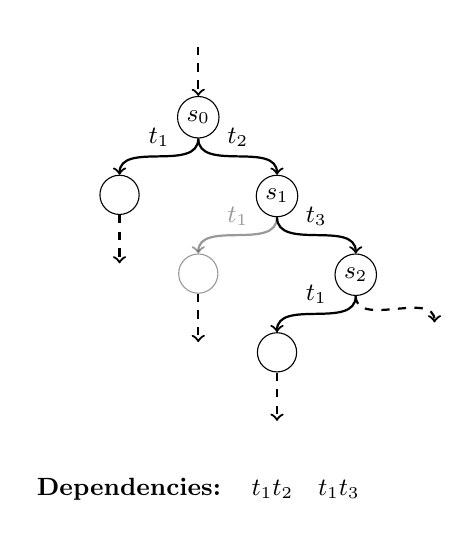
\begin{tikzpicture}[ball/.style = {circle, draw, align=center, anchor=north, inner sep=0, text width=0.5cm}]
    \node[ball]              (A) at (0,0)   {\small $s_0$};
    \node[ball]              (B) at (-1,-1) {};
    \node[ball]              (C) at (1,-1)  {\small $s_1$};
    \node[ball, opacity=0.4] (D) at (0,-2)  {};
    \node[ball]              (E) at (2,-2)  {\small $s_2$};
    \node[ball]              (F) at (1,-3)  {};

    \node (init) at (0,0.75)   {};
    \node (end1) at (-1,-2.25) {};
    \node (end2) at (0,-3.25)  {};
    \node (end3) at (3,-3)     {};
    \node (end4) at (1,-4.25)  {};
    \draw[->, thick, draw, dashed] (init.south) to [out=270,in=90] (A.north);
    \draw[->, thick, draw, dashed] (B.south) to [out=270,in=90] (end1.north);
    \draw[->, thick, draw, dashed] (D.south) to [out=270,in=90] (end2.north);
    \draw[->, thick, draw, dashed] (E.south) to [out=270,in=90] (end3.north);
    \draw[->, thick, draw, dashed] (F.south) to [out=270,in=90] (end4.north);

    \draw[->, thick, draw]              (A.south) to [out=270,in=90] node[midway,above] {\small $t_1$} (B.north);
    \draw[->, thick, draw]              (A.south) to [out=270,in=90] node[midway,above] {\small $t_2$} (C.north);
    \draw[->, thick, draw, opacity=0.4] (C.south) to [out=270,in=90] node[midway,above] {\small $t_1$} (D.north);
    \draw[->, thick, draw]              (C.south) to [out=270,in=90] node[midway,above] {\small $t_3$} (E.north);
    \draw[->, thick, draw]              (E.south) to [out=270,in=90] node[midway,above] {\small $t_1$} (F.north);

    \node (note) at (0,-5) {
      \small \textbf{Dependencies:} \hspace{0.1cm} $t_1 \independent t_2$ \hspace{0.1cm} $t_1 \dependent t_3$
    };
  \end{tikzpicture}
  \caption[The sleep set optimisation.]{The sleep set optimisation.  Transition $t_1$ may be pruned in state $s_1$ but not in state $s_2$.  The transition has been explored from state $s_0$ and there is no dependent transition between states $s_0$ and $s_1$, but there is between states $s_0$ and $s_2$.  Adapted from \cite{coons2013}.}\label{fig:sleep}
\end{figure}

\paragraph{Sleep sets}
The sleep set optimisation \parencite{godefroid1996} is a complementary
approach to DPOR which we use to further reduce schedules explored.
The intuition is as follows: if we are in a state $s_{0}$ and have a
choice of two scheduling decisions, $t_{1}$ and $t_{2}$, after trying
out $t_{1}$ there is no point in making the sequence of decisions
$t_{2}t_{1}$ from $s_{0}$, unless $t_{1} \dependent t_{2}$.  All
states reachable from $t_{1}$ have already been explored, so the only
way a new state could arise is if $t_{1}$ had a different effect,
which will only be the case if a dependent transition has been taken.
\Cref{fig:sleep} shows this graphically.

Formally, we augment each state $s$ with a \emph{sleep set},
containing transitions enabled in $s$ but which we will not make.  The
initial state has an empty sleep set.  Let $T$ be the transitions that
have been selected to be explored from $s$.  We proceed as follows:
take a transition $t_{1}$ out of $T$.  The sleep set associated with
the state reached after executing $t_{1}$ from $s$ is the sleep set
associated with $s$, minus all transitions that are dependent with
$t_{1}$.  Let $t_{2}$ be a second transition taken out of $T$.  The
sleep set associated with the state reached after executing $t_{2}$
from $s$ is the sleep set associated with $s$ augmented with $t_{1}$,
minus all transitions that are dependent with $t_{2}$.  We continue
until all transitions in $T$ have been explored, at each step adding
the previously taken transitions to the sleep set of the new state,
and removing the dependent transitions.

\paragraph{Schedule bounding}
\dejafu{} supports pre-emption bounding \parencite{musuvathi2007}; fair
bounding \parencite{musuvathi2008}; and depth, or length,
bounding \parencite{russell2002}.  We use a variant of the bounded
partial-order reduction algorithm~(BPOR) \parencite{coons2013}, augmented
with support for relaxed memory \parencite{zhang2015}, as our core testing
algorithm.  All three bounds are enabled by default, but can be
selectively disabled or changed.

\paragraph{Daemon threads}
A daemon thread is a thread which is automatically killed after the
last non-daemon thread terminates.  In Haskell, every thread other
than the main thread is a daemon thread, so as soon as the main thread
terminates the whole program terminates.  This is a problem for DPOR,
as it makes the last action of the execution dependent with everything
else in the program!

\begin{listing}
\centering
\begin{cminted}{haskell}
main = do
  v <- newEmptyMVar
  fork (myThreadId >> putMVar v "hello world")
  tryReadMVar v
\end{cminted}
\caption{A program with a race condition.}\label{lst:daemon1}
\end{listing}

\Cref{lst:daemon1} has two results: \verb|Nothing|, and
\verb|Just "hello world"|.  However, there is no dependency between
\verb|myThreadId| and \verb|tryReadMVar|, so if the scheduler favours
the main thread, we do not see the other result.  Introducing a
dependency between the last action of the execution and everything
else solves this problem.

\begin{listing}
\centering
\begin{cminted}{haskell}
main = do
  v <- newEmptyMVar
  fork (myThreadId >> myThreadId >> putMVar v "hello world")
  tryReadMVar v
\end{cminted}
\caption{Another program with a race condition.}\label{lst:daemon2}
\end{listing}

However, these new dependencies also present a difficulty.  In
\Cref{lst:daemon2}, the forked thread now performs \verb|myThreadId|
twice.  If the \verb|tryReadMVar| happens after the second of these,
we get the same result as if it happens after the first.  Normally,
DPOR would recognise this and prune the redundant decision, as
\verb|myThreadId| and \verb|tryReadMVar| are independent.  However, by
introducing a dependency between the final action and everything else,
we have said that it is \emph{not} redundant!  In general, introducing
a dependency like this will lead to many redundant executions which we
would otherwise avoid.

The solution we adopt is to change the scheduler.  If the scheduler
has a choice of actions, where one or more will cause the main thread
to terminate, it records each decision as a backtracking point.  By
ensuring that every decision is tried at least once, we do not need to
introduce an additional dependency between the final action of the
main thread and everything else, and can just let DPOR do its job as
usual.

\section{Execution traces}
\label{sec:dejafu-traces}

Execution traces are not the easiest of things to read, especially if
there are many context switches.  Traces generated by random
scheduling are particularly difficult to read, which is unfortunate,
as random testing with a fixed number of executions can be effective
for finding bugs and is much faster than DPOR.

\dejafu{} contains a trace simplifier, which attempts to rewrite
traces into a shorter form.  Unlike the shrinking done in tools like
QuickCheck \parencite{claessen2000}, \dejafu{}'s trace simplification is
\emph{semantics-preserving}.  An execution trace can be rewritten into
a simpler form which is guaranteed to produce the same result, and
there is no need to run the program again to verify this.  We achieve
this by only re-ordering independent actions, using the dependency
relation.

\begin{listing}
\begin{sublisting}{\textwidth}
\centering
\begin{cminted}{text}
S0-----P1--P0-P1-S0-P2--C-S0---P2-P3-P2--S3-P0-P3-P0---S3-P0-P3-S0-
S0----P1-P0-----P2--P0--P2-P0-S2--S3-P1-P0---S1-S3----S0--
S0--------P2-P0--P3-P2-P0-P3-P2-C-S0-S3---S2--S1-C-S1-P0----
\end{cminted}
\caption{Original}\label{lst:trace_simplification_orig}
\end{sublisting}

% [layout hack]: no gap between the listings otherwise
\vspace{1.5em}

\begin{sublisting}{\textwidth}
\centering
\begin{cminted}{text}
S0----------P1---S2-----S0----S3-----S0--
S0----------P1-P2-----S0--S1--S0---S3-----S0--
S0----------P2--P3-----S0--S2---S1--P0----
\end{cminted}
\caption{Simplified}\label{lst:trace_simplification_simplified}
\end{sublisting}
\caption[The effect of trace simplification.]{Three execution traces produced by random scheduling and their simplified counterparts.}\label{lst:trace_simplification}
\end{listing}

\Cref{lst:trace_simplification} shows three execution traces generated
by random scheduling, from a test of \dejafu{}'s relaxed memory
implementation.  These traces are displayed in a pretty-printed form
which gives just the essence of the scheduling decisions:

\begin{itemize}
\item \verb|Sn|: indicates that thread \verb|n| started executing
  after the previously executing thread blocked or terminated.
\item \verb|Pn|: indicates that thread \verb|n| started executing by
  pre-empting the previously executing thread.
\item \verb|pn|: indicates that thread \verb|n| started executing
  after the previously executing thread yielded or delayed.
\item \verb|C|: indicates the execution of a relaxed memory commit.
\item \verb|-|: indicates the execution of one primitive action.
\end{itemize}

The three original traces involve many context
switches and relaxed memory commit actions.  They are long and hard to
follow.  In contrast, the three simplified traces are much shorter,
involve far fewer context switches, and have no relaxed memory commit
actions at all.  The simplified traces are much more useful for
program comprehension.

Our trace simplification algorithm has four steps:

\begin{enumerate}
\item Rewrite the trace into lexicographic normal form.
\item Prune redundant relaxed memory commit actions.
\item Reduce context switching by pulling actions backwards.
\item Reduce context switching by pushing actions forwards.
\end{enumerate}

We repeat steps (3) and (4) until a fixed point is reached, or a fixed
number of iterations has elapsed.

\paragraph{Rewrite the trace into lexicographic normal form}
The problem of sorting sequences where only some items can be permuted
is studied in \cite{anisimov1979}.  For the case of execution traces,
this corresponds to sorting by thread identifier, only re-ordering
independent actions.  We implement this in much the same way as bubble
sort.

Recall that a Haskell program terminates when the main thread does.
So by moving actions of the main thread, thread 0, towards the
beginning we can delete a suffix of the trace.

\paragraph{Prune redundant relaxed memory commit actions}
If a commit action is followed by a memory barrier, possibly with some
independent actions in between, the commit can be removed if there are
no other buffered writes for that \verb|IORef|.  The barrier will
commit the single write anyway.

\paragraph{Reduce context switching by pulling actions backwards}
We now walk through the trace from beginning to end, looking for
opportunities to pull actions backwards.  If we have the trace
\verb|[(t1, X), (t2, Y), (t1, Z)]|, where \verb|Y| and \verb|Z| are
independent, the this transformation re-orders the trace to
\verb|[(t1, X), (t1, Z), (t2, Y)]|.  We allow arbitrary separations,
as long as all of the actions in the middle are independent with the
action being pulled backwards.

\paragraph{Reduce context switching by pushing actions forwards}
This is much like the ``pull back'' transformation.  We walk the
trace, looking for cases where actions can be pushed forward.  If we
have the trace \verb|[(t1, X), (t2, Y), (t1, Z)]|, where \verb|X| and
\verb|Y| are independent, this transformation re-orders the trace to
\verb|[(t2, Y), (t1, X), (t1, Z)]|.

The ``pull back'' and ``push forward'' transformations are not
inverses of each other, as the dependency relation is not transitive.
It may be that an action \verb|X| can be pushed forward to just before
an action \verb|Z|, but \verb|Z| could not be pulled back to just
after \verb|X|.

\section{Soundness and Completeness}
\label{sec:dejafu-correctness}

Correctness for \dejafu{} divides along a natural separation in the
theory: correctness of a single execution of a concurrent program, and
correctness of the testing framework which discovers new executions.
There is also the concern of correctness of the implementation with
respect to the theory.  We do not attempt to formally verify the
implementation, but we do have an extensive test suite.  Testing a
testing tool is a little different to testing a regular program.  Most
of our tests consist of nondeterministic programs, where we want to
verify that \dejafu{} finds precisely the behaviours we expect.

\paragraph{Property tests}
\dejafu{} is not one monolithic implementation.  It has components
which can be specified and tested in isolation.  For example, the
dependency relation must be commutative.  We use
Hedgehog \parencite{hedgehog}, a randomised property-testing library, to
check these properties of the implementation.

\paragraph{Integration tests}
Most of the tests are integration tests, consisting of a small
concurrent program and a property to check.  A failure in such an
integration test could in principle be anywhere in \dejafu{}, and so
be hard to isolate and fix, but in practice failures in different
components tend to manifest differently.  For example, a failure in
the DPOR implementation tends to manifest as invalid schedules being
generated; whereas a failure in the concurrency implementation tends
to manifest as incorrect results.

Our integration tests fall into the following classes:

\begin{itemize}
\item Single threaded tests for the \verb|MonadConc| primitives,
  ensuring that only the single correct behaviour is observed.
\item Multi-threaded tests for the \verb|MonadConc| primitives,
  ensuring that the expected nondeterminism is observed.
\item So-called \emph{litmus tests} for the relaxed memory
  implementation, ensuring that all expected relaxed behaviours are
  observed.
\item A copy of the async library's \parencite{async} test suite, for our
  \verb|MonadConc| version.
\item A collection of refinement tests from CoCo, which we shall
  discuss in \Cref{chp:coco}.
\item Finally, a collection of regression tests for previous bugs.
\end{itemize}

\paragraph{Example programs}
Finally, we have a collection of larger integration tests which serve
also as example usages of \dejafu{}, three of which we discuss in
\Cref{sec:dejafu-casestudies}: the auto-update
library \parencite{auto_update}, the monad-par
library \parencite{monad_par,marlow2011}, and the async library \parencite{async}.

\subsection{Correct Execution}

Correctness of execution asks: can the result of an arbitrary
execution of \dejafu{}'s testing implementation can be obtained in
reality?  Furthermore, do all real-world executions correspond to a
possible execution under \dejafu{}?

\paragraph{Program behaviour}
There is no standard for concurrent Haskell.  There is only what GHC
provides.  The behaviour of many operations is clear, but for some it
is not.  \verb|IORef| operations are particularly complicated, as their
behaviour depends on the underlying memory model, which is
unspecified.  We chose TSO, and assume that the GHC optimiser or code
generator does not affect the memory model.

There are some intentional semantic differences for practical reasons.
For example, GHC can sometimes detect deadlocks involving only a
subset of the threads, and throw an exception to the threads
signalling this.  We cannot do this.

Although the behaviour of \dejafu{} is not correct with respect to
GHC-compiled behaviour in all cases, we claim it is close enough to be
useful.

\paragraph{Possible executions}
Our stepwise execution of concurrent programs allows a scheduling
decision to be made between each primitive action, which does not
correspond to how GHC handles scheduling:

\begin{displayquote}
  GHC implements pre-emptive multitasking: the execution of threads
  are interleaved in a random fashion.  More specifically, a thread may
  be pre-empted whenever it allocates some memory, which unfortunately
  means that tight loops which do no allocation tend to lock out other
  threads (this only seems to happen with pathological benchmark-style
  code, however). \parencite{control_concurrent}
\end{displayquote}

So there are executions involving the pre-emption of the evaluation of
non-terminating expressions which are possible under GHC but not under
\dejafu{}.  However, \dejafu{} is even worse than this with bottom
values.  The program in \Cref{lst:bottom} will fail to terminate, even
if the thread with the infinite computation is never scheduled, as
\dejafu{} will hang trying to compute the continuation so it can call
the scheduler.

\begin{listing}
\centering
\begin{cminted}{haskell}
bottom = do
  fork (last [1..])
  pure ()
\end{cminted}
\caption{A program that does not halt under \dejafu{} but does under GHC.}\label{lst:bottom}
\end{listing}

\subsection{Correct Testing}

Correctness of testing asks: are the schedule prefixes generated by
the DPOR machinery valid?  Furthermore, are there any possible results
for which no schedule will be generated?  This is different to the
testing framework generating every schedule, as that is precisely what
DPOR tries to avoid.

\paragraph{Prefix validity}
Executions are stored internally as a stack, shown in \Cref{lst:dpor}.
The sequence of thread IDs corresponding to this stack represents a
complete execution of the program.  There is a unique initial state,
where only the initial thread is runnable and nothing has been done.

\begin{listing}
\centering
\begin{cminted}{haskell}
data DPOR = DPOR
  { dporRunnable :: Set ThreadId
  -- ^ What threads are runnable at this step.
  , dporTodo     :: Map ThreadId Bool
  -- ^ Follow-on decisions still to make, and whether that decision
  -- was added conservatively due to the bound.
  , dporNext     :: Maybe (ThreadId, DPOR)
  -- ^ The next decision made.
  , dporDone     :: Set ThreadId
  -- ^ All transitions which have been taken from this point,
  -- including conservatively-added ones.
  , dporSleep    :: Map ThreadId ThreadAction
  -- ^ Transitions to ignore until a dependent transition happens.
  , dporTaken    :: Map ThreadId ThreadAction
  -- ^ Transitions which have been taken, excluding
  -- conservatively-added ones.
  } deriving (Eq, Show)
\end{cminted}
\caption{The DPOR state is a stack of scheduling decisions.}\label{lst:dpor}
\end{listing}

There are some well-formedness properties associated with a
\verb|DPOR| value:

\begin{enumerate}
\item Every thread in the to-do set is runnable.
\item Every thread in the done set is runnable.
\item The taken set is a subset of the done set.
\item The done and to-do sets are disjoint.
\item The next-taken thread, if there is one, is in the done set.
\end{enumerate}

These properties should hold inductively over the whole state.  We
check these invariants everywhere a \verb|DPOR| value is constructed,
and abort if the state is invalid.  In the \dejafu{} testsuite, the
execution time overhead of this checking is 3\%.

The prefixes we generate are sequences of taken decisions followed by
a single to-do decision.  By maximising the length of prefixes, we
obtain a depth-first search of the space of schedules.  Provided the
well-formedness properties hold, and the runnable sets are correctly
recorded during execution, then a generated schedule prefix will be
valid.

\paragraph{Schedule completeness}
The DPOR machinery should eventually find every possible result of a
given program.  However, as schedule bounding is involved, some
results may not be reached.  So instead we require that, for all sets
of bounds, all results possible subject to those bounds show up under
testing with the same bounds.  Our core testing algorithm satisfies
this property \parencite{coons2013}.

\section{Case Studies}
\label{sec:dejafu-casestudies}

We now discuss the process and results of applying \dejafu{} to three
Haskell libraries:

\begin{enumerate}
\item We reproduce a known deadlock in the auto-update
  library \parencite{auto_update}.
\item We identify and fix a deadlock in the monad-par
  library \parencite{monad_par,marlow2011}.
\item We use property-based testing to reproduce a known bug in the
  async library \parencite{async}.
\end{enumerate}

We chose these libraries because each is by proficient Haskell
programmers well versed with concurrency, and yet they all contain
unintentional bugs.  This shows that even those familiar with the
standard pitfalls of concurrent programming encounter problems.

None of these libraries is written using the \verb|MonadConc|
abstraction, so we had to modify the existing code before we could
test them with \dejafu{}.

\subsection{auto-update}

The auto-update library \parencite{auto_update} runs tasks periodically, but
only if needed.  For example, a web server may handle each request in
a new thread, and log the time that the request arrives.  Rather than
have every such new thread check the time, one thread could be created
to update a single shared \verb|IORef| every second.  However, if the
request frequency is less than once per second, this is wasted work.
The library allows defining a periodic action which only runs when
needed.

The implementation, excluding comments and imports, is reproduced in
\Cref{lst:autoupdate}.  The library defines a function,
\verb|mkAutoUpdate|, which forks a worker thread to perform the action
when required.  The function returns an \verb|IO| action to read the
current result, if necessary blocking until there is one.  The
transformation to the \verb|MonadConc| typeclass is straightforward,
and we omit it here.

\begin{listing}
\centering
\begin{cminted}{haskell}
test_autoupdate :: MonadConc m => m ()
test_autoupdate = do
  auto <- mkAutoUpdate defaultUpdateSettings
  auto
\end{cminted}
\caption{An example usage of the auto-update library.}\label{lst:autoupdate_example1}
\end{listing}

\Cref{lst:autoupdate_example1} shows an example usage of the
\verb|MonadConc| version of the library.  The
\verb|defaultUpdateSettings| value describes an auto-updater which
runs every second, producing the value \verb|()|.  An \verb|MVar| is
used to communicate to the thread that the updater should run.  Inside
the worker, a delay is used to ensure that the action is not computed
too frequently: this is what gives the rate limiting.  So we create an
auto-updater which produces \verb|()|, and immediately demand the
value.

\begin{listing}
\centering
\begin{cminted}{text}
> autocheck test_autoupdate

[fail] Never Deadlocks
        [deadlock] S0--------S1-----------S0-
[pass] No Exceptions
[fail] Consistent Result
        () S0--------S1--------p0--

        [deadlock] S0--------S1-----------S0-
\end{cminted}
\caption[Using \dejafu{} to run a collection of standard tests.]{Using \dejafu{} to run a collection of standard tests.  The \texttt{autocheck} function looks for deadlocks, uncaught exceptions in the main thread, and nondeterminism.  Each result is displayed with a simplified view of a representative execution trace.}\label{lst:autoupdate_example2}
\end{listing}

\paragraph{Testing with \dejafu{}}
\Cref{lst:autoupdate_example2} shows one way in which we can use
\dejafu{} to explore the behaviour of our small example.  The
\verb|autocheck| function looks for some common concurrency errors.
In this example, \dejafu{} discovers a deadlock.  Each result is
displayed with a simplified view of a representative execution trace.
More detailed execution traces are also available, which contain a
summary of the primitive actions which occurred and the alternative
scheduling decisions available.

We can see from the trace of the deadlock result that thread 0
executed for a while, then thread 1, then thread 0 again.  As these
are all \verb|S| points, each thread executed until it blocked.  So we
can look at the source code in \Cref{lst:autoupdate_example1} and
\Cref{lst:autoupdate} to see what happened.

Following the execution by eye, we see this sequence of concurrency
events:

\begin{enumerate}
\item Thread 0:
  \begin{enumerate}
  \item Line 16: \verb|currRef <- newIORef Nothing|
  \item Line 17: \verb|needsRunning <- newEmptyMVar|
  \item Line 18: \verb|lastValue <- newEmptyMVar|
  \item Line 20: \verb|void $ forkIO $ ...|
  \item Line 35: \verb|mval <- readIORef currRef|
  \item Line 39: \verb|void $ tryPutMVar needsRunning ()|
  \item Line 40: \verb|readMVar lastValue|
  \item \textbf{Thread 0 is now blocked, as \texttt{lastValue} is empty.}
  \end{enumerate}
\item Thread 1:
  \begin{enumerate}
  \item Line 21: \verb|takeMVar needsRunning|
  \item Line 25: \verb|writeIORef currRef $ Just a|
  \item Line 26: \verb|void $ tryTakeMVar lastValue|
  \item Line 27: \verb|putMVar lastValue a|
  \item \textbf{Thread 0 is now unblocked, as \texttt{lastValue} is full.}
  \item Line 29: \verb|threadDelay $ updateFreq us|
  \item Line 31: \verb|writeIORef currRef Nothing|
  \item Line 32: \verb|void $ takeMVar lastValue|
  \item \textbf{Thread 0 is still unblocked, even though \texttt{lastValue} is now empty again.}
  \item \textbf{Thread 1 now loops.}
  \item Line 21: \verb|takeMVar needsRunning|
  \item \textbf{Thread 1 is now blocked, as \texttt{needsRunning} is empty.}
  \end{enumerate}
\item Thread 0:
  \begin{enumerate}
  \item Line 40: \verb|readMVar lastValue|
  \item \textbf{Thread 0 is now blocked, as \texttt{lastValue} is empty.}
  \end{enumerate}
\end{enumerate}

Both threads are blocked, so the computation is deadlocked.  The other
result shown in \Cref{lst:autoupdate_example2} occurs if thread 0
starts executing after thread 1 delays.  So the root cause of this
deadlock is clear: deadlock may occur if the call to
\verb|threadDelay| on line 29 completes before the other thread
resumes execution.  Despite this bug being rather simple, not
requiring any pre-emptions at all to trigger, it arose in practice.
How easy it is to make mistakes when implementing concurrent programs!

\begin{table}
  \centering
  \begin{subtable}{\textwidth}
    \centering
    \begin{tabular}{lSSSS} \toprule
      & {Schedules} & {Deadlocks} & {Time (s)} & {Max Residency (kB)} \\ \midrule
      Bounded DPOR   &  49 & 18 & 0.006 &  119 \\
      Unbounded DPOR &  80 & 20 & 0.008 &  124 \\
      Swarm          & 100 & 20 & 0.008 & 1297 \\ \bottomrule
    \end{tabular}
    \caption{Keeping all execution traces in memory.}\label{tbl:autoupdate_perf1}
  \end{subtable}

  % [layout hack]: no gap between the tables otherwise
  \vspace{1.5em}

  \begin{subtable}{\textwidth}
    \centering
    \begin{tabular}{lSSSS} \toprule
      & {Schedules} & {Deadlocks} & {Time (s)} & {Max Residency (kB)} \\ \midrule
      Bounded DPOR   &  49 & 18 & 0.006 &  71 \\
      Unbounded DPOR &  80 & 20 & 0.006 &  63 \\
      Swarm          & 100 & 20 & 0.006 & 108 \\ \bottomrule
    \end{tabular}
    \caption{Only keeping buggy execution traces in memory.}\label{tbl:autoupdate_perf2}
  \end{subtable}
  \caption[Performance of the auto-update case study with multiple strategies.]{Performance of the auto-update case study with three different exploration tactics.}\label{tbl:autoupdate_perf}
\end{table}

\paragraph{Performance of testing}
\Cref{tbl:autoupdate_perf} shows performance measurements for our test
case in six different configurations: three different algorithms to
explore the space of schedules, keeping or discarding execution
traces.  Both the library itself and our test case are small, so it is
perhaps no surprise to see that in all configurations, execution only
takes a fraction of a second.  We can see the effect of the schedule
bounding: when the bounds are disabled, the number of schedules tried
almost doubles, and two new deadlocking executions are found.

To reduce memory usage, \dejafu{} is able to discard results or
execution traces which the user considers uninteresting in some way.
\Cref{tbl:autoupdate_perf2} shows the impact of this change, where we
have designated non-deadlocking traces as uninteresting.  The effect
is particularly significant in the Swarm case, suggesting that Swarm
may tend to find longer execution traces than DPOR.

\begin{listing}
  \centering
  \begin{minipage}{0.5\textwidth}
  \begin{minted}[linenos]{haskell}
data UpdateSettings a = UpdateSettings
    { updateFreq           :: Int
    , updateSpawnThreshold :: Int
    , updateAction         :: IO a
    }

defaultUpdateSettings :: UpdateSettings ()
defaultUpdateSettings = UpdateSettings
    { updateFreq           = 1000000
    , updateSpawnThreshold = 3
    , updateAction         = return ()
    }

mkAutoUpdate :: UpdateSettings a -> IO (IO a)
mkAutoUpdate us = do
    currRef      <- newIORef Nothing
    needsRunning <- newEmptyMVar
    lastValue    <- newEmptyMVar

    void $ forkIO $ forever $ do
        takeMVar needsRunning

        a <- catchSome $ updateAction us

        writeIORef currRef $ Just a
        void $ tryTakeMVar lastValue
        putMVar lastValue a

        threadDelay $ updateFreq us

        writeIORef currRef Nothing
        void $ takeMVar lastValue

    pure $ do
        mval <- readIORef currRef
        case mval of
            Just val -> return val
            Nothing -> do
                void $ tryPutMVar needsRunning ()
                readMVar lastValue

catchSome :: IO a -> IO a
catchSome act = catch act $
  \e -> pure $ throw (e :: SomeException)
  \end{minted}
  \end{minipage}
  \caption{The implementation of the auto-update package.}\label{lst:autoupdate}
\end{listing}

% [layout hack]: get lst:autoupdate here.
\FloatBarrier

\subsection{monad-par}
\label{sec:dejafu-casestudies-par}

The monad-par library \parencite{monad_par,marlow2011} provides a
traditional-looking concurrency abstraction, giving the programmer
threads and mutable state, however it is deterministic.  Determinism
is enforced by restricting shared state: it is an error to write more
than once to the same mutable variable, and read operations block
until a value has been written.  Programs written using the library
will either give a deterministic result, or terminate with a
multiple-write error.  These shared variables, called \verb|IVar|s,
implement futures \parencite{marlow2011}.  Despite its limitations, the
library can be effective in speeding up pure code \parencite{marlow2011}.

The library provides six different schedulers.  We ported the
``direct'' scheduler, a work-stealing scheduler, to the
\verb|MonadConc| typeclass.  This was a straightforward and
compiler-driven refactoring.  Changing function types to use
\verb|MonadConc| rather than \verb|IO| led to compiler errors showing
where the next changes needed to be made.  We iterated this process of
fixing errors and recompiling until the library successfully compiled
once more.  Changes were needed in two of the source files.

Some simplifications were made in the conversion process:

\begin{itemize}
\item The scheduler creates a pseudorandom number generator for each
  worker thread.  As systematic testing requires that the scheduler be
  the only source of nondeterminism, we fixed the random seeds: the
  first worker thread gets the seed zero, the second gets the seed
  one, and so on.
\item The scheduler uses the C pre-processor to choose between
  different implementations of some of its functionality.  There are
  nine flags, each of which are independent.  We only ported and
  tested the default configuration.
\item The scheduler includes some debugging code for detecting and
  reporting errors.  We removed it.
\end{itemize}

\begin{table}
  \centering
  \begin{tabular}{lrr} \toprule
    & Direct.hs & DirectInternal.hs \\ \midrule
    Language extensions & 1 & 0 \\
    Module imports & 6 & 1 \\
    Type definitions & 7 & 13 \\
    Type signatures & 32 & 7 \\
    Function renames & 2 & 0 \\
    Logic changes & 16 & 0 \\ \midrule
    \emph{Total} & 75 & 26 \\ \bottomrule
  \end{tabular}
  \caption{Breakdown of changes to port the monad-par ``direct'' scheduler.}\label{tbl:parmonad_diff}
\end{table}

\Cref{lst:parmonad} shows the original and converted versions of the
scheduler initialisation code.  As can be seen, they are similar, even
though this is a core component of a rather sophisticated library,
where the types have been changed.  \Cref{tbl:parmonad_diff} breaks
down the changes across both files.  Code changes are broken down into
``renames,'' where the concurrency library simply provides a different
name for a function, and ``logic,'' where that was not the case.  The
logic changes were either: (1) places where a call to \verb|liftIO| or
\verb|lift| was now necessary; or (2) inserting uses of
\verb|getNumCapabilities|.

\begin{listing}
\centering
\begin{cminted}{haskell}
parfilter :: (MonadConc m, NFData a) => (a -> Bool) -> [a] -> Par m [a]
parfilter _ []  = pure []
parfilter f [x] = pure (if f x then [x] else [])
parfilter f xs  = do
    let (as, bs) = halve xs
    v1 <- Par.spawn (parfilter f as)
    v2 <- Par.spawn (parfilter f bs)
    left  <- Par.get v1
    right <- Par.get v2
    pure (left ++ right)
  where
    halve xs = splitAt (length xs `div` 2) xs
\end{cminted}
\caption{An example usage of the monad-par library.}\label{lst:parmonad_example1}
\end{listing}

\Cref{lst:parmonad_example1} shows an example usage of the library.
This \verb|parfilter| function filters a list in parallel, using a
divide-and-conquer approach.  If the list is not empty or a singleton,
it is split in half and a new thread created to filter each half.  The
results of each new thread are combined to produce the overall result.
The library requires all shared state have an instance of the
\verb|NFData| typeclass, which provides an operation to evaluate data
to normal form.  The library gains its speed by evaluating data in
separate threads.

\begin{listing}
\centering
\begin{cminted}{haskell}
test_parmonad :: (MonadConc m, MonadIO m) => [Int] -> m Bool
test_parmonad xs = do
    let p x = x `mod` 2 == 0
    s <- runPar (parfilter p xs)
    pure (s == filter p xs)
\end{cminted}
\caption{A test case comparing a parallel filter to a normal filter.}\label{lst:parmonad_example2}
\end{listing}

\paragraph{Finding a deadlock}
\Cref{lst:parmonad_example2} shows a test case for \verb|parfilter|.
A parallel filter should produce the same result as a normal filter.
\Cref{tbl:parmonad_perf} shows performance measurements for our test
case, with the input list \verb|[0..5]|, in six different
configurations.  The numbers do not look so good for DPOR.  Swarm
managed to find two deadlocking executions out of 100, whereas bounded
DPOR found none in 6140.  Unbounded DPOR did not complete at all: it
rapidly consumed all the memory of the host system when keeping traces
in memory, and was still running after two days while discarding
traces.

\begin{table}
  \centering
  \begin{subtable}{\textwidth}
    \centering
    \begin{tabular}{lSSSS} \toprule
      & {Schedules} & {Deadlocks} & {Time (s)} & {Max Residency (MB)} \\ \midrule
      Bounded DPOR   & 6140 & 0 & 35.1 &            339 \\
      Unbounded DPOR &      &   &      & {$\geq$ 16GiB} \\
      Swarm          &  100 & 2 & 0.17 &             21 \\ \bottomrule
    \end{tabular}
    \caption{Keeping all execution traces in memory.}\label{tbl:parmonad_perf1}
  \end{subtable}

  % [layout hack]: no gap between the tables otherwise
  \vspace{1.5em}

  \begin{subtable}{\textwidth}
    \centering
    \begin{tabular}{lSSSS} \toprule
      & {Schedules} & {Deadlocks} & {Time (s)} & {Max Residency (kB)} \\ \midrule
      Bounded DPOR   & 6140 & 0 &           27.9 &  842 \\
      Unbounded DPOR &      &   & {$\geq$ 48hrs} &      \\
      Swarm          &  100 & 2 &           0.14 & 1600 \\ \bottomrule
    \end{tabular}
    \caption{Only keeping buggy execution traces in memory.}\label{tbl:parmonad_perf2}
  \end{subtable}
  \caption[Performance of the monad-par case study with multiple strategies.]{Performance of the monad-par case study with three different exploration tactics.  Unbounded DPOR was aborted in both cases, after consuming too many resources.}\label{tbl:parmonad_perf}
\end{table}

When we inspect one of the execution traces leading to deadlock, we
gain two clues for why DPOR performs poorly: (1) the trace is 793
entries long, but the length bound for DPOR is 250; and (2) there are
473 calls to \verb|liftIO|, \dejafu{} considers all \verb|IO| actions
dependent and so tries every possible interleaving of these.

\begin{listing}
\centering
\begin{cminted}{text}
(Continue,[],LiftIO)
(Continue,[],LiftIO)
(Continue,[],LiftIO)
(Continue,[],ReadIORef 2)
(Continue,[],LiftIO)
(Continue,[],NewMVar 7)
(Continue,[],ModIORef 4)
(Continue,[],GetNumCapabilities 2)
(Continue,[],BlockedTakeMVar 7)
\end{cminted}
\caption{The final ten entries of the deadlocking monad-par trace.}\label{lst:parmonad_example3}
\end{listing}

Following the code by eye as we read a 793-entry trace is not a
feasible approach here.  So instead, let's look at the last few
entries in the trace, shown in \Cref{lst:parmonad_example3}.  Each
trace entry is a tuple consisting of: the scheduling decision made,
the alternative decisions possible, and what the thread did.  As this
is right before deadlock, it is not surprising that there are no other
threads which could be scheduled.  There are only four calls to
\verb|getNumCapabilities| in the code we ported.  So we can look at
each, to find one where the surrounding context matches the trace.

\begin{listing}
\centering
\begin{cminted}{haskell}
go 0 _ | _IDLING_ON =
  do m <- newEmptyMVar
     r <- modifyHotVar idle (\is -> (m:is, is))
     numCapabilities <- getNumCapabilities
     if length r == numCapabilities - 1
       then do
         mapM_ (\vr -> putMVar vr True) r
       else do
         done <- takeMVar m
         if done
           then do
             return ()
           else do
             i <- getnext (-1::Int)
             go (maxtries numCapabilities) i
\end{cminted}
\caption[The source of the deadlock in the monad-par library.]{The source of the deadlock in the monad-par library.  In the ``then'' branch of the conditional, the \texttt{idle} list is not emptied when waking every blocked thread.}\label{lst:parmonad_example4}
\end{listing}

\Cref{lst:parmonad_example4} is our match.  When a thread is unable to
steal work, it creates an empty \verb|MVar| which it adds to a shared
list, called \verb|idle|; if that list already has an entry for every
other thread, they are woken by writing a value to their \verb|MVar|;
otherwise, the thread blocks by calling \verb|takeMVar| on its new,
empty, \verb|MVar|.

The final fragment of our execution trace corresponds to this code
where the condition \verb|length r == numCapabilities - 1| is false.
But how can that be false?  \emph{The list is never emptied!}  Think
about what happens if every thread reaches this logic \emph{twice}:

\begin{enumerate}
\item \verb|n - 1| threads add themselves to the list, and block.
\item The final thread adds itself to the list, and wakes up the other
  threads.
\item \textbf{The list is not emptied, even though every thread is woken.}
\item \verb|n - 1| threads add themselves to the list, again, and
  block.
\item The final thread adds itself to the list.  It does \emph{not}
  trigger the wake-up logic, because the list is not the right length,
  and so it also blocks.
\item \textbf{Every thread is now blocked.}
\end{enumerate}

We can confirm our suspicion by checking the trace.  Each thread does
exhibit that pattern twice, so our deduction is correct.  This problem
is solved by writing \verb|[]| to \verb|idle| before waking the
threads.  The write must happen before, otherwise there is a new race
condition: one of the woken threads could add itself to the list
again, and then its \verb|MVar| be lost when the list is cleared.

\paragraph{Handling an exception}
When running our test case in a loop using \verb|IO|, to verify that
we really had fixed the problem, another issue arose which \dejafu{}
did \emph{not} find.  After a while, the main thread would be killed
by a \verb|BlockedIndefinitelyOnMVar| exception.  Such exceptions are
out of scope~\sref{dejafu-scope}, so \dejafu{} could never find this
new problem.

By turning on the library's debugging output, and adding some more of
our own, we were able to track the problem down to the same logic as
before, \Cref{lst:parmonad_example4}.  A thread was still getting
blocked here, despite our fix for the deadlock.  How can a thread get
blocked indefinitely there if we make sure the last thread wakes up
the others?  \emph{The number of workers is assumed to be equal to the
  number of capabilities!}  If even a single worker terminates, all
the others will block.

Fortunately, the relevant source code is not extensive.  We were able
to quickly ascertain that the library divides its workers into two
categories: there is a single main worker, which communicates the
result of the computation back to its caller and terminates when done;
and there are all the other workers.  The other workers do check if
the computation is complete, but only in certain places.  So this was
happening:

\begin{enumerate}
\item A non-main worker checks if the computation is complete, and
  sees that it is not.
\item The same worker blocks itself as usual.
\item The computation finishes, and the main worker terminates.
\item \textbf{The GHC runtime delivers an exception to the blocked
    worker.}
\end{enumerate}

It is harmless for the worker to be blocked at this point, as the
overall computation is long-complete, and the result communicated back
to the user.  However, each worker thread is given an exception
handler which throws any received exception to its creator.  In this
case, the creator was the main thread, so the whole program is
terminated.  The solution is to check if the computation has
terminated before blocking.

\paragraph{Two different concurrency bugs}
The second problem appears to be far more prevalent under normal
execution than the deadlock, which requires an unfair schedule.  This
shows that just using \dejafu{} is not enough, it is always possible
to have such an out of scope bug which \dejafu{} cannot find for you.

Fixes for both issues have been merged into the monad-par library.

\begin{listing}
  \begin{sublisting}{\textwidth}
    \centering
    \begin{cminted}{haskell}
makeScheds :: Int -> IO [Sched]
makeScheds main = do
   workpools <- replicateM numCapabilities $ R.newQ
   rngs <- replicateM numCapabilities $ Random.create >>= newHotVar
   idle <- newHotVar []
   sessionFinished <- newHotVar False
   sessionStacks   <- mapM newHotVar
     (replicate numCapabilities [Session baseSessionID sessionFinished])
   activeSessions  <- newHotVar S.empty
   sessionCounter  <- newHotVar (baseSessionID + 1)
   let allscheds = [ Sched { no=x, idle, isMain=(x==main), workpool=wp,
                             scheds=allscheds, rng=rng, sessions=stck
                             sessionCounter, activeSessions
                           }
                   | x   <- [0 .. numCapabilities-1]
                   | wp  <- workpools
                   | rng <- rngs
                   | stck <- sessionStacks
                   ]
   pure allscheds
    \end{cminted}
    \caption{Original}\label{lst:parmonad_orig}
  \end{sublisting}

  % [layout hack]: no gap between the listings otherwise
  \vspace{1.5em}

  \begin{sublisting}{\textwidth}
    \centering
    \begin{cminted}{haskell}
makeScheds :: (MonadConc m, MonadIO m) => Int -> m [Sched m]
makeScheds main = do
   numCapabilities <- getNumCapabilities
   workpools <- replicateM numCapabilities $ liftIO R.newQ
   let rng i = liftIO (Random.initialize (V.singleton $ fromIntegral i))
   rngs <- mapM (\i -> rng i >>= newHotVar) [0..numCapabilities]
   idle <- newHotVar []
   sessionFinished <- newHotVar False
   sessionStacks   <- mapM newHotVar
     (replicate numCapabilities [Session baseSessionID sessionFinished])
   activeSessions  <- newHotVar S.empty
   sessionCounter  <- newHotVar (baseSessionID + 1)
   let allscheds = [ Sched { no=x, idle, isMain=(x==main), workpool=wp,
                             scheds=allscheds, rng=rng, sessions=stck
                             sessionCounter, activeSessions
                           }
                   | x   <- [0 .. numCapabilities-1]
                   | wp  <- workpools
                   | rng <- rngs
                   | stck <- sessionStacks
                   ]
   pure allscheds
    \end{cminted}
    \caption{\dejafu{}}\label{lst:parmonad_dejafu}
  \end{sublisting}
  \caption{The monad-par ``direct'' scheduler initialisation.}\label{lst:parmonad}
\end{listing}

% [layout hack]: get lst:parmonad here.
\FloatBarrier

\subsection{async}
\label{sec:dejafu-casestudies-async}

The async library \parencite{async} allows programmers to write asynchronous
code without needing to worry about details such as threads, shared
state, or exceptions.  \Cref{lst:async_example} shows a typical usage
of the library.  The \verb|async| function begins executing an
\verb|IO| action in a new thread.  The \verb|wait| function blocks
until the action is done and returns the result.  If the action throws
an exception, \verb|wait| also throws the exception.  There is a third
basic operation: \verb|cancel|, which terminates the thread associated
with an asynchronous action.

\begin{listing}
\centering
\begin{cminted}{haskell}
downloadBoth :: URL -> URL -> IO (String, String)
downloadBoth url1 url2 = do
  a1 <- async (download url1)
  a2 <- async (download url2)
  page1 <- wait a1
  page2 <- wait a2
  pure (page1, page2)
\end{cminted}
\caption[A typical usage of the async library.]{A typical usage of the async library.  Both URLs are downloaded concurrently in separate threads.}\label{lst:async_example}
\end{listing}

Using these three building blocks of \verb|async|, \verb|wait|, and
\verb|cancel|, the library provides a collection of higher-level
abstractions which are widely used in the Haskell ecosystem.  One of
these higher-level abstractions is the \verb|Concurrently| type, a
simple wrapper around \verb|IO|, which allows concurrently composing
actions with the \verb|Applicative| \verb|<*>| operator.  The two
arguments to \verb|<*>| are computed concurrently in separate threads,
and then combined.  \Cref{lst:concurrently} gives the implementation
of \verb|Concurrently|.

In Haskell, we like our typeclasses to have \emph{laws} specifying how
instances should behave.  Without such a specification, it is
impossible to write typeclass-polymorphic functions with any
reasonable expectation of what will happen.  These laws are not
checked by the compiler: GHC is no theorem prover.  Rather, it is up
to the author of a typeclass instance to ensure that they follow all
appropriate laws.  Failure by a library author to follow the laws can
lead to unexpected behaviour for users.  As \verb|Applicative| is a
superclass of \verb|Monad|, it should come as no surprise that there
is a law relating the two: specifically, that \verb|<*> = ap|.  The
definition of \verb|ap| is given in \Cref{lst:ap}.

\begin{listing}
\centering
\begin{cminted}{haskell}
ap :: Monad m => m (a -> b) -> m a -> m b
ap f a = do
  f' <- f
  a' <- a
  pure (f' a')
\end{cminted}
\caption{The \texttt{ap} function.}\label{lst:ap}
\end{listing}

The \verb|ap| law does \emph{not} hold for the \verb|Concurrently|
monad\footnote{\url{https://github.com/simonmar/async/pull/26}}!  With
the benefit of hindsight, the cause is clear: \verb|<*>| runs its
arguments concurrently, whereas \verb|ap| has no choice but to run its
arguments sequentially.  If the two arguments can concurrently
interfere with each other, then \verb|<*>| exhibits more
nondeterminism than \verb|ap|.

\paragraph{Property-testing typeclass laws}
Could \dejafu{} have helped here?  We believe so.  By changing the
\verb|Concurrently| type to be polymorphic over the underlying monad,
we can substitute in any \verb|MonadConc|.  We can then test the laws.
We used QuickCheck \parencite{claessen2000} for this, but any
property-testing tool which can generate functions and check monadic
properties would do.

\begin{listing}
\centering
\begin{cminted}{haskell}
prop_monad_ap1 :: Ord b => Fun a b -> a -> Property
prop_monad_ap1 (apply -> f) a = (pure f <*> pure a) `eq` (pure f `ap` pure a)

eq :: Ord a => Concurrently ConcIO a -> Concurrently ConcIO a -> Property
eq (Concurrently left) (Concurrently right) = monadicIO $ do
  l <- resultsSet defaultWay defaultMemType left
  r <- resultsSet defaultWay defaultMemType right
  assert (l == r)
\end{cminted}
%$
\caption{The \texttt{<*> = ap} law, with no concurrent interference.}\label{lst:aplaw1}
\end{listing}

\Cref{lst:aplaw1} shows a \emph{passing} property.  There is no
concurrent interference between the two arguments to \verb|<*>| and
\verb|ap|, so the bug does not manifest.  Our \verb|eq| function
checks that two \verb|Concurrently| actions produce the same sets of
results.  For the reader unfamiliar with \verb|QuickCheck|:
\verb|Fun a b| represents a function of type \verb|a -> b|; and
\verb|monadicIO| converts an \verb|IO| action into a test which passes
if it contains no failing assertions.

Our \verb|prop_monad_ap1| property is uninteresting in a sense because
it is clearly free from concurrency errors: the very errors which we
want to detect!  It is free of them because the arguments to
\verb|<*>| and \verb|ap| are pure values, so there can be no
concurrent interference between them.  To observe the law being
broken, we must create a race condition.

\begin{listing}
\centering
\begin{cminted}{haskell}
prop_monad_ap2 :: Ord b => Fun a b -> Fun a b -> a -> Property
prop_monad_ap2 (apply -> f) (apply -> g) a = go (<*>) `eq` go ap where
  go combine = do
    flagvar <- newEmptyMVar
    let cf = do { flag <- tryPutMVar flagvar (); pure (if flag then f else g) }
    let ca = do { tryPutMVar flagvar (); pure a }
    pure (Concurrently cf `combine` Concurrently ca)
\end{cminted}
\caption{The \texttt{<*> = ap} law, with concurrent interference.}\label{lst:aplaw2}
\end{listing}

\Cref{lst:aplaw2} contains a race condition.  We now generate two
functions with QuickCheck.  When executing the concurrent action, we
use an \verb|MVar| to decide which function to use.  If the
\verb|MVar| is empty we use the first function, if it is full we use
the second.  If the combining function, \verb|<*>| or \verb|ap|,
executes its arguments concurrently we will see both functions tried;
if it executes its arguments sequentially, we will only see the first
function.  Indeed, we do see the bug.  \Cref{lst:aplaw3} gives the
QuickCheck and \dejafu{} outputs.

\begin{listing}
\begin{sublisting}{\textwidth}
\centering
\begin{cminted}{text}
> quickCheck prop_monad_ap2
*** Failed! Falsifiable (after 3 tests and 8 shrinks):
{_->""}
{_->"a"}
0
\end{cminted}
\caption{The QuickCheck output.}\label{lst:aplaw3_quickcheck}
\end{sublisting}

% [layout hack]: no gap between the listings otherwise
\vspace{1.5em}

\begin{sublisting}{\textwidth}
\centering
\begin{cminted}{text}
> resultSet defaultWay defaultMemType (go (<*>) (\_ -> "") (\_ -> "a") 0)
fromList [Right "",Right "a"]

> resultSet defaultWay defaultMemType (go ap (\_ -> "") (\_ -> "a") 0)
fromList [Right "a"]
\end{cminted}
\caption{The \dejafu{} output.}\label{lst:aplaw3_dejafu}
\end{sublisting}
\caption{The result of the failing \texttt{<*> = ap} property.}\label{lst:aplaw3}
\end{listing}

\paragraph{Performance of testing}
\Cref{tbl:concurrently_perf} shows performance measurements for a
variant of our test case.  We cannot give the property itself to
\dejafu{}, so we extract the \verb|MonadConc| computation and
hard-code the parameters generated by QuickCheck, shown in
\Cref{lst:concurrently_example}.  As in the auto-update case study,
this is a small test case, so it is perhaps unsurprising that it is
fast and requires little memory.  Once again, we see that Swarm
requires more memory than DPOR, even taking the increased number of
schedules tried into account.

\paragraph{The benefit of hindsight}
We have the benefit of knowing about the bug, leading us to the
correct test.  Is it unrealistic to expect a user to have the
foresight to write a test like this in the beginning?  We think not.
When implementing functions for combining concurrent actions, it is no
great leap to wonder what happens if there are races between these
actions.  The property may appear contrived, but it is a natural way
to investigate the effect of a race condition in the \verb|<*> = ap|
law.

\begin{table}
  \centering
  \begin{subtable}{\textwidth}
    \centering
    \begin{tabular}{lSSSS} \toprule
      & {Schedules} & {Failures} & {Time (s)} & {Max Residency (kB)} \\ \midrule
      Bounded DPOR   &  17 &  2 & 0.002 &  131 \\
      Unbounded DPOR &  30 &  3 & 0.004 &  135 \\
      Swarm          & 100 & 37 & 0.012 & 1360 \\ \bottomrule
    \end{tabular}
    \caption{Keeping all execution traces in memory.}\label{tbl:concurrently_perf1}
  \end{subtable}

  % [layout hack]: no gap between the tables otherwise
  \vspace{1.5em}

  \begin{subtable}{\textwidth}
    \centering
    \begin{tabular}{lSSSS} \toprule
      & {Schedules} & {Failures} & {Time (s)} & {Max Residency (kB)} \\ \midrule
      Bounded DPOR   &  17 &  2 & 0.004 &  92 \\
      Unbounded DPOR &  30 &  3 & 0.009 &  85 \\
      Swarm          & 100 & 37 & 0.011 & 648 \\ \bottomrule
    \end{tabular}
    \caption{Only keeping buggy execution traces in memory.}\label{tbl:concurrently_perf2}
  \end{subtable}
  \caption[Performance of the \texttt{<*> = ap} test case.]{Performance of the \texttt{<*> = ap} test case with three different exploration tactics.}\label{tbl:concurrently_perf}
\end{table}

\begin{listing}
\centering
\begin{cminted}{haskell}
test_concurrently :: MonadConc m => m Bool
test_concurrently = do
    l <- go (<*>)
    r <- go ap
    pure (l == r)
  where
    go combine = runConcurrently $ do
      flagvar <- newEmptyMVar
      let cf = do { flag <- tryPutMVar flagvar (); pure (if flag then f else g) }
      let ca = do { tryPutMVar flagvar (); pure a }
      pure (Concurrently cf `combine` Concurrently ca)

    f = \_ -> ""
    g = \_ -> "a"
    a = 0
\end{cminted}
%$
\caption{The \texttt{<*> = ap} test case, with the generated functions hard-coded.}\label{lst:concurrently_example}
\end{listing}

\begin{listing}
\centering
\begin{cminted}{haskell}
newtype Concurrently a = Concurrently { runConcurrently :: IO a }

instance Functor Concurrently where
  fmap f (Concurrently a) = Concurrently (fmap f a)

instance Applicative Concurrently where
  pure = Concurrently . pure

  Concurrently fs <*> Concurrently as =
    Concurrently (fmap (\(f, a) -> f a) (concurrently fs as))

instance Monad Concurrently where
  return = pure

  Concurrently a >>= f =
    Concurrently (a >>= runConcurrently . f)

concurrently :: IO a -> IO b -> IO (a, b)
concurrently left right = concurrently' left right (collect []) where
  collect [Left a, Right b] _ = pure (a, b)
  collect [Right b, Left a] _ = pure (a, b)
  collect xs m = do
    e <- takeMVar m
    case e of
      Left ex -> throw ex
      Right r -> collect (r:xs) m

concurrently'
  :: IO a
  -> IO b
  -> (MVar (Either SomeException (Either a b)) -> IO r)
  -> IO r
concurrently' left right collect = do
  done <- newEmptyMVar
  mask $ \restore -> do
    let run a r = restore (a >>= putMVar done . Right . r)
                  `catch` (putMVar done . Left)
    lid <- fork (run left  Left)
    rid <- fork (run right Right)
    let stop = killThread rid >> killThread lid
    r <- restore (collect done) `onException` stop
    stop
    pure r
\end{cminted}
%$
\caption{The implementation of the \texttt{Concurrently} type.}\label{lst:concurrently}
\end{listing}

% [layout hack]: get lst:concurrently here.
\FloatBarrier

\section{Evaluation}
\label{sec:dejafu-evaluation}

A tool is effectively useless if it is too difficult to use.  The main
obstacle to the use of \dejafu{} is existing libraries which use
\verb|IO|; a programmer cannot simply use \verb|liftIO| everywhere,
without sacrificing completeness in all but simple cases.  Ideally,
existing libraries would be modified to support the \verb|MonadConc|
abstraction.  However, this does not seem a likely short-term goal,
and so a more promising way to approach the problem is to provide
alternatives to existing libraries.  As adapting code to
\verb|MonadConc| is often straightforward, as seen in the monad-par
case study~\sref{dejafu-casestudies-par}, this is a viable solution.

\paragraph{Users}
Although \dejafu{} is a small one-man project, it does have some users
and contributors.  Ten users have opened issues on the GitHub issue
tracker; a further three have asked me for help over IRC and email;
and six have made small contributions.  Two features came directly
from user requests, motivated by performance concerns in large test
cases: (1) random scheduling, which we discuss further in
\Cref{chp:algorithms}; and (2) the ability to discard uninteresting
results or execution traces as they are discovered, before evaluating
the predicate at the end.  This second feature can have a significant
impact.  If you are interested in a particular failure, it is much
better to discard those results which \emph{do not} exhibit the
failure as they are discovered, rather than keep them around in memory
until the end.  \Cref{fig:discard} shows the effect of this on a
simple test of \verb|MVar| contention.

\begin{figure}
  \centering
  \begin{subfigure}{0.49\textwidth}
    \centering
    \includegraphics[width=\textwidth]{fig/nodiscard.png}
    \caption{Keeping all results and traces in memory.}
  \end{subfigure}
  \begin{subfigure}{0.49\textwidth}
    \centering
    \includegraphics[width=\textwidth]{fig/discard.png}
    \caption{Discarding all traces, just keeping results.}
  \end{subfigure}
  \caption[Heap profiles of a test case for \texttt{MVar} contention.]{Heap profiles of a test case for \texttt{MVar} contention.  Note the dramatic difference: 250M without discarding vs 60k with.  These plots are intended to be viewed with colour.}\label{fig:discard}
\end{figure}

Tweag I/O\footnote{\url{http://www.tweag.io/}}, a research and
development company based in Paris, are using \dejafu{} as part of
their work on a distributed system for the SAGE
project\footnote{\url{http://www.sagestorage.eu/}}, which is
investigating storage systems for future supercomputers.  They cannot
share details of their work for commercial reasons, but one developer
had this to say (emphasis mine):

\begin{displayquote}
  Regarding the test case: we have an implementation of a distributed
  storage cluster, with possibly many nodes and parallel requests.
  The storage system itself is composed of several layers, which can
  be stacked on top of one another.  There is a lot of asynchronicity
  involved.  As per the tests themselves, I am testing parallel
  requests over different objects, etc.

  \emph{I'd like to add that dejafu tests are by far the most reliable
    tests in our suite, in my experience - I am yet to see a
    concurrency bug that they didn't spot, while some other tests
    missed them!} \parencite{tweag2017}
\end{displayquote}

\subsection{Richness of the Abstraction}

As we noted in \Cref{sec:dejafu-scope}, there are some areas which we
do not currently aim to support with \dejafu{}:

\begin{itemize}
\item Blocking a thread until a file descriptor becomes available, as
  this introduces an additional source of nondeterminism.
\item Throwing an exception to a thread if it becomes deadlocked, as
  we cannot reliably detect deadlock involving only a subset of
  threads without support from the garbage collector.
\item Querying which capability (OS thread) a Haskell thread is
  running on, as this introduces an additional source of
  nondeterminism.
\end{itemize}

These three areas are out of scope because we believe that the desire
for this functionality does not outweigh the implementation cost.  We
will look for a way, if that belief changes.

Introducing additional sources of nondeterminism into an SCT model is
difficult.  Simply introducing additional threads to model the
nondeterminism can cause an explosion of schedules tested, which is
unsatisfactory.  \verb|MonadConc| will always be limited to what
\dejafu{} can reasonably support.

However we can still push back the boundaries of what \dejafu{} supports.
Bound threads, Haskell threads which always run on the same unique OS
thread, were once out of scope as well.  This made it impossible to
use some C libraries with \verb|MonadConc|.  Now we have a prototype
implementation\footnote{\url{https://github.com/barrucadu/dejafu/issues/126}}
which shows promise, and which we intend to release.

\subsection{Writing and Porting Class-polymorphic Code}

\begin{listing}
\centering
\begin{cminted}{haskell}
instance MonadLogger (LoggerT STM) where -- ...
instance MonadLogger (LoggerT IO) where -- ...
\end{cminted}
\caption{Concrete instances for a typeclass-based logging abstraction.}\label{lst:mlogger1}
\end{listing}

We saw in the Par monad example that porting complex code to the
\verb|MonadConc| abstraction is not necessarily a difficult process.
However, this is not always the case.  Recently a user tried to port a
logging abstraction they made to \verb|MonadConc|.  Expressing this
with \verb|MonadConc| and \verb|MonadSTM| is not straightforward, as
constraints do not factor into instance selection.  So the instances
in \Cref{lst:mlogger2} overlap, and are illegal in standard Haskell.

\begin{listing}
\centering
\begin{cminted}{haskell}
instance MonadSTM  m => MonadLogger (LoggerT m) where -- ...
instance MonadConc m => MonadLogger (LoggerT m) where -- ...
\end{cminted}
\caption{Overlapping instances for a typeclass-based logging abstraction.}\label{lst:mlogger2}
\end{listing}

After some work, we introduced new \verb|IsSTM| and \verb|IsConc|
types to disambiguate between the two cases, and ended up with
\Cref{lst:mlogger3}.  The amount of effort required to arrive at this
solution led to the user questioning whether classes like their
\verb|MonadLogger| were even a useful abstraction at
all\footnote{\url{https://www.reddit.com/r/haskell/comments/7b1fbk/do_mtlstyle_effect_classes_really_pull_their/}}!
This is a good topic to think about, but it should not be prompted by
the effort of trying to use \dejafu{}.

\begin{listing}
\centering
\begin{cminted}{haskell}
instance MonadSTM  m => MonadLogger (LoggerT (IsSTM  m)) where -- ...
instance MonadConc m => MonadLogger (LoggerT (IsConc m)) where -- ...
\end{cminted}
\caption{Polymorphic instances for a typeclass-based logging abstraction.}\label{lst:mlogger3}
\end{listing}

So while porting code to the \verb|MonadConc| typeclass is often
simple when dealing with datatype and function definitions, it can be
more complicated when dealing with typeclasses.  It is not clear what
can be done to improve this matter.

\subsection{Library Alternatives}

There are popular Haskell libraries specifically for concurrency.  One
of these is the async library \parencite{async}, part of which we looked at
as a case study~\sref{dejafu-casestudies-async}, for expressing
asynchronous computations.  This library is intended to be a
higher-level and safer way of expressing asynchronous computations
with guaranteed cleanup than using threading, mutable state, and
asynchronous exceptions directly.

Our concurrency library \parencite{concurrency}, which provides
\verb|MonadConc|, includes an alternative to async using
\verb|MonadConc|.  There is a test suite using \dejafu{}.  The test
suite for async itself just runs most tests a single time, although
one of them is run 1000 times.  Using \dejafu{} here to automatically
seek out interesting schedules is a much more principled approach then
repetition and hope.  Not all features of async are supported,
however.  As we do not currently support bound threads, functions that
use them have been omitted.

This is just one library, and providing an alternative library that
people will have to switch to is far from optimal.  However, until
library authors start to use \dejafu{} and \verb|MonadConc| directly,
such alternatives will be needed to answer the question `Why should I
use this if I cannot use it with anything I use already?'

\subsection{Tool Integration}

There are two popular libraries for unit testing in Haskell,
HUnit \parencite{hunit} and Tasty \parencite{tasty}.  From the perspective of the
user, the libraries are similar, but from the perspective of the
implementer, they have different approaches to integration.  The
hunit-dejafu \parencite{hunit_dejafu} and tasty-dejafu \parencite{tasty_dejafu}
packages provide integration with both.

These packages provide analogues of the \dejafu{} functions, but using
the interface of the testing frameworks, rather than computing and
printing results directly.  The test-framework \parencite{test_framework}
library is also in common use, however it supports integration with
HUnit, and so needs no special support of its own.

The Tasty library is more featureful than HUnit, supporting progress
reporting, giving a message on success as well as failure, and
command-line arguments.  The tasty-dejafu package is similar to the
hunit-dejafu package and does not make use of these additional
features.

% \section{Conclusions}
% \label{sec:dejafu-conclusions}

% Although a commonly reported experience amongst Haskell programmers is
% that `if it compiles, it works,' there are times where it does
% \emph{not} work.  Concurrency is a particularly difficult area to get
% right, as everyone who has had to move outside the realm of guaranteed
% determinism will know.  A number of profiling and debugging tools
% exist, typically requiring special runtime support.  Yet there are no
% debugging tools for concurrent Haskell programs.  We contribute such a
% tool, at the cost of a programmer having to use a generalisation of
% the familiar concurrency abstraction.

% This work was inspired by attending a talk at INVEST 2014 by Paul
% Thompson, then a Ph.D student at Imperial College London, on
% systematic concurrency testing, the talk mentioned tools for languages
% like Java and C, but functional languages were not mentioned at all.
% The questions to be answered, then, were:

% \begin{itemize}
% \item \textbf{Can concurrency testing techniques from the imperative
%     and object-oriented worlds be applied in the functional world?}
%   \hfill

%   The answer to this would seem to be a resounding `yes.'  There was
%   some difficulty in implementing these techniques in a purely
%   functional setting, as the algorithms are typically expressed in
%   terms of mutable state, but this was overcome.

% \item \textbf{Does the purely functional setting allow for new
%     techniques to be developed?} \hfill

%   At first we hoped that the lack of effects in evaluation, amongst
%   other things, would allow for new techniques to be developed.
%   However, as concurrency testing explicitly cares about
%   \emph{execution} rather than \emph{evaluation} (although these are
%   one and the same in most languages), this does not seem to be the
%   case.
% \end{itemize}

% In \cite{walker2015}, we asked if the cost of a programmer needing to
% write their code in terms of \verb|MonadConc| rather than \verb|IO|
% was too high, and would discourage people.  This is still a concern,
% but with the development of libraries to integrate with or replace
% others, we hope that the use of \dejafu{} will appear attractive
% enough to overcome this.

% The contributions of this work are:

% \begin{itemize}
% \item a generalisation of a large subset of the GHC concurrency
%   abstraction;

% \item a library called \dejafu{} for the systematic and random testing
%   of concurrent Haskell programs, including those using relaxed-memory
%   effects; and

% \item a convincing demonstration that systematic concurrency
%   techniques work well in a rich concurrency setting such as Haskell.
% \end{itemize}

\vfill\pagebreak
\section{Summary}

In this chapter we presented \dejafu{}, our tool for testing
concurrent Haskell programs:

\begin{itemize}
\item We provide a typeclass abstraction over concurrency.  Such an
  abstraction allows \verb|IO| to be swapped out and replaced with
  another implementation~\sref{dejafu-monadconc}.

\item We implemented a model of Haskell
  concurrency~\sref{dejafu-execution}, with an empirically derived
  operational semantics~\sref{dejafu-semantics}, so that we can
  simulate the behaviour of GHC.  Our model includes most of the
  Control.Concurrent library module, although some operations are out
  of scope, or have their behaviour changed~\sref{dejafu-scope}.

\item We use bounded partial-order reduction \parencite{coons2013} with
  relaxed memory \parencite{zhang2015} as the core testing algorithm for
  \dejafu{}, but also support a controlled random scheduling
  approach~\sref{dejafu-testing}.

\item We have not attempted a formal proof of correctness of
  \dejafu{}, but have made an informal correctness argument, noting
  the limits of how correct \dejafu{} can be.  We do have a
  comprehensive test suite, and check what correctness conditions we
  can~\sref{dejafu-correctness}.

\item We have discussed three case studies, all of which involved
  applying \dejafu{} to pre-existing code.  Such code must be modified
  to use the \dejafu{} typeclass abstraction, but we have found this
  to be a straightforward and type-directed process in most
  cases~\sref{dejafu-casestudies}.
\end{itemize}

Although a commonly reported experience amongst Haskell programmers is
that ``if it compiles, it works,'' there are times when it does
\emph{not} work.  Concurrency is a particularly difficult area to get
right, as everyone who has had to move outside the realm of guaranteed
determinism will know.  By developing \dejafu{}, we hope that
concurrency in Haskell will become a little easier to get right.

\paragraph{Context}
\dejafu{} does not stand alone, it is related to our other
contributions:

\begin{itemize}
\item \Cref{chp:algorithms} discusses a new random scheduling
  algorithm for incomplete concurrency testing.  The chapter does not
  directly build on \dejafu{}, but \dejafu{} implements the algorithm.
\item \Cref{chp:coco} discusses a new property-discovery tool for
  functions operating on mutable state.  The tool directly builds on
  \dejafu{} in two ways: (1) to discover these properties, and (2) by
  providing an interface for \dejafu{} to check them.
\end{itemize}


  \section{Evaluation of Results}
  \label{sec:progress-evaluation}
  Something I care about in my research is that any tools or theoretical
work I produce be applicable to real-world problems. If a tool has
beautiful properties in principle, but takes a day to run on anything
but tiny problems, that is not good enough.

\paragraph{Is it new?}

If a tool offers \emph{nothing} new over an existing one, nobody will
use it. More pertinently, without novelty, it's not research. Novelty
doesn't have to mean a completely new approach, it can equally be a
combination of prior ideas into a form which hasn't been explored
before. A proxy for this is publications. Direct comparison with other
tools with the same aim can also serve.

\paragraph{Is it sound?}

Formal verification is the gold standard, but it's not the only way to
be confident of soundness. Comparison with other tools and use of
standard test cases can be used to seek out any discrepancies.

\paragraph{is it complete?}

If the tool says there is no bug, is that actually true? \dejafu{}
already sacrifices completeness, but it should be complete within the
chosen bounds. For concurrency testing tools, incompleteness is likely
to manifest as false negatives, and so can be accounted for in the
same way as soundness: use of standard test cases and comparison with
other tools.

\paragraph{Is it practical?}

Does the tool finish running in a reasonable time on real-world
examples? Can the programmer use it without large modification to
their code? There are standard benchmarks for concurrency testing
tools which can be used to measure performance, allowing comparison
with similar tools for other languages. Lines of code changed, as
shown in the Par monad example in the attached technical report, can
serve as a proxy for the amount of work a programmer needs to do
before using a tool.

\paragraph{Does it suggest further work?}

Finally, is there any potential for further development? Limitations
can suggest where algorithmic improvements could possibly be made.


\chapter{Research Plan}
\label{chp:plan}
This chapter describes the test execution of a concurrent program
written using the \verb|MonadConc| abstraction, not the execution of
programs using GHC's actual concurrency primitives. Of course, for
correctness of testing, there should be a correspondence between these
two models, see \chap{correctness}.

The execution of a concurrent program is considered to be the
sequential stepwise execution of \emph{primitive actions}, the most
basic things that a computation can do.


  \section{\dejafu{} Journal Article}
  \label{sec:plan-journal}
  \dejafu{} has been developed substantially since \citep{dejafu}. The
published version is very slow and lacking in features in
comparison. A fuller and updated account is being prepared (see the
supporting document). In the short-term, I plan to continue improving
that document and submit it for consideration as an official
departmental technical report. The longer-term plan is to continue
improving the document and submit it to a journal for publication.

Perhaps the natural choice of venue is the Journal of Functional
Programming, as \dejafu{} is for testing concurrent \emph{Haskell}
programs, and is implemented in Haskell. But there may be other more
suitable ones, which must be investigated.

\paragraph{Timeline:}

\begin{description}
\item[End of Feb 2016] Submit for consideration as a departmental
  technical report.

\item[End of Mar 2016] Submit to a journal.
\end{description}

\paragraph{Success Criteria:}

A journal article is accepted.


  \section{Live Property Monitoring}
  \label{sec:plan-ltl}
  Runtime Verification (RV) is a broad field concerned with integrating
techniques from program verification with analysis of data gathered
from real-world executions of programs. The advantage of runtime
verification is that many static analyses are necessarily
\emph{undecidable} or \emph{inefficient} in general, however
restricting interest to a particular execution often allows further
optimisation and analysis to be done.

An example of this is DPOR. Partial-order reduction is a purely
static-analysis based method. DPOR is considered to be an
\emph{optimisation} as it can often use the data gathered at run-time
about dependencies between actions to do less overall work
\citep{dpor}.

\emph{Linear Temporal Logic} (LTL) is a popular logic in the field of
runtime verification for formulating and checking properties of
programs \citep{ltl}. There has been prior work on checking LTL
properties of concurrent Haskell programs \citep{hsrv}, but this work
appears not to have been developed further. In particular, the authors
do not integrate their work with any sort of systematic testing
framework. This allows violations of properties to be detected in
individual real-world executions, but does not allow for searching for
violations.

LTL is an extension of propositional logic with the ability to reason
about \emph{time}. For checking properties of programs, this means
that the formula-verifier has access to an execution trace. There are
four additional operators:

\begin{description}
\item[$p~\mathbf{U}~q$ (``$p$ until $q$'')] $p$ must hold (at least)
  until $q$ does. $q$ must become true eventually.

\item[$\mathbf{X}~p$ (``next $p$'')] $p$ holds in the next time step.

\item[$\mathbf{F}~p$ (``in the future $p$'')] $p$ holds at some future
  point.

\item[$\mathbf{G}~p$ (``globally $p$'')] $p$ always holds.
\end{description}

Writing a tool which uses \dejafu{} to check LTL properties of
concurrent programs would allow the systematic search for violations
of complex run-time invariants. An example given in \citep{hsrv} is
detecting the presence of lock reversal (acquiring a pair of locks in
one order and then using them in the other order), which \emph{can}
cause deadlock. It is nice to be able to detect that an invariant
violation occurs at run-time, it would be nicer to be able to detect
it during testing.

There are two ways to approach this. Either this property checking
could be performed as the computation is executed, aborting execution
when a violation occurs; or, the execution trace could be examined
after-the-fact for property violations. It is not immediately obvious
which is better.

\paragraph{Timeline:}

\begin{description}
\item[End of Apr 2016] Have a tool capable of checking LTL properties
  against all executions of a concurrent program under \dejafu{},
  showing failing schedules.
\item[Mid May 2016] Submit a paper to the International Conference on
  Runtime Verification.
\end{description}

\paragraph{Success Criteria:}

The tool is able to, for each execution, prove or disprove a LTL
formula where possible; to return a new formula if complete evaluation
was not possible; and to report failing executions.

\paragraph{Publications:}

If successful, this should result in a paper being submitted to the
2016 International Conference on Runtime Verification.


  \section{Test Case Generation}
  \label{sec:plan-quickspec}
  \dejafu{} allows the testing of concurrent programs, but these test
cases still need to be written. It can be hard to think of good test
cases for concurrent systems, as bugs are typically caused by the
pre-emption of a thread where this is not expected. As programmers are
bad at recognising this situation, it is also difficult to
deliberately try to provoke it.

QuickSpec \citep{quickspec} is a tool for generating laws that a
collection of functions appear to hold based on random testing. It can
be used as a way to obtain suitable test cases, if the user selects
the generated laws that \emph{should} hold, rather than those which
merely \emph{accidentally} hold. Furthermore, the \emph{absence} of
expected laws can often hint at the presence of a bug which further
testing can reveal.

A QuickSpec-like tool which can generate laws for a concurrency-using
API would be interesting and useful. Ideally the programmer would
supply a description of some collection of functions, and the tool
would generate small concurrent programs and find properties of their
results.

For example, given a concurrent stack type, it would be desirable to
be able to generate both of these properties automatically:

\begin{haskellcode}
do { s <- newStack; push s 1; push s 2; a <- pop s; b <- pop s; return (a, b) }
  `gives` {(2,1)}

do { s <- newStack; push s 1 <|> push s 2; a <- pop s; b <- pop s; return (a, b) }
  `gives` {(2,1), (1,2)}
\end{haskellcode}

Where \verb|gives| produces the set of results of a concurrent
computation and \verb+<|>+ is parallel composition. Such properties
can serve as small simple test cases, and the basis of a larger test
suite.

There are a few problems with QuickSpec which make it unsuitable for
this task currently:

\begin{itemize}
\item QuickSpec cannot generate $\lambda$-functions directly, which
  makes it of limited use when generating properties involving monadic
  bind, \verb|(>>=)|.

\item QuickSpec generates ``small'' functions, and slows down
  significantly as the size bound is increased. However, interesting
  properties of concurrent data structures are likely to involve
  several function calls monadically composed.
\end{itemize}

One possible approach may be from the angle of generating do-notation
code one line at a time, rather than generating expressions in
generality. As we are interested in properties of monadic things only,
this alternative view may provide new insights, and allow restricting
the search space.

\paragraph{Timeline:}

\begin{description}
\item[End of Jun 2016] Have a prototype tool which can generate
  type-correct monadic expressions in do-notation style from a
  collection of provided functions.

\item[End of Aug 2016] Support concurrency and relate generated
  expressions to properties over sets of possible results.
\end{description}

\paragraph{Success Criteria:}

The tool is capable of generating expected properties of concurrent
implementations of stacks, queues, binary heaps, maps, and any other
data structures of interest. Properties exhibiting race conditions and
deadlocks should be generated where they exist.

\paragraph{Publications:}

I believe that this would be worthy of a paper. However, this will not
be finished in time. A submission in 2017 would be feasible.

\paragraph{Future Research:}

Most of the difficulty in implementing this tool will be the
combinatorial explosion of possible type-correct expressions. Trying
to cut down on this should be a rich area to explore. One possible
avenue is attempting to find heuristics to bias the search towards
more ``interesting'' properties, sacrificing completeness for speed.


  \section{Concurrency Introduction}
  \label{sec:plan-searchparty}
  The \emph{Search Party}\footnote{\github{barrucadu}{search-party}}
library supports speculative parallelism in generate-and-test search
problems. It is motivated by the consideration that: if multiple
acceptable solutions exist, it may not matter which one is
returned. Initially, only single results could be returned, but
support for returning all results was later added, incorrectly,
introducing a bug.

The key piece of code causing the problem was this part of the worker
loop:

\begin{minted}{haskell}
case maybea of
  Just a -> do
    atomically $ do
      val <- tryTakeCTMVar res
      case val of
        Just (Just as) -> putCTMVar res $ Just (a:as)
        _ -> putCTMVar res $ Just [a]
    unless shortcircuit $
      process remaining res
  Nothing -> process remaining res
\end{minted}

Here \verb|maybea| is a value indicating whether the computation just
evaluated was successful. The intended behaviour is that, if a
computation is successful, its result is added to the list in the
\verb|res| \verb|CTMVar|. This \verb|CTMVar| is exposed indirectly to
the user of the library, as it is blocked upon when the final result
of the search is requested.

There are some small tests in \emph{Search Party}, verifying that
deadlocks and exceptions don't arise, and that results are as
expected. Upon introducing this new functionality, tests began to fail
with differing result lists returned for different schedules,
prompting the test:\footnote{The \texttt{representative} function
  picks only one trace for each unique result.}

\begin{minted}{haskell}
checkResultLists :: Eq a => Predicate [a]
checkResultLists = representative (alwaysTrue2 check) where
  check (Right (Just as)) (Right (Just bs)) = as `elem` permutations bs
  check a b = a == b
\end{minted}

Given this predicate, we can very clearly see the problem:

\begin{verbatim}
> dejafu (runFind $ [0..2] @! const True) ("Result Lists", checkResultLists)

[fail] Result Lists (checked: 145)
        Just [0] S0-----S1---------S3-------S0-------
        Just [1] S0-----S1---------S3---P2-------S0-------
        Just [1,0] S0-----S1---------S3-------S2-------S0-------
        Just [0,1] S0-----S1---------S3---P2-------S3----S0-------
False
\end{verbatim}

The problem was a lack of any indication that a list-producing
computation had finished. As results were written directly to the
\verb|CTMVar|, partial result lists could be read depending on how the
worker threads and the main thread were interleaved.

In this case, fixing the failure did not require any interactive
debugging. Only one place had been modified in introducing the new
functionality, and the bug was found by re-reading the code with the
possibility of error in mind. However, the ability to produce a test
case which reliably reproduces the problem gives confidence that it
will not be accidentally reintroduced.


  \section{Types}
  \label{sec:plan-types}
  Static type systems can be thought of as a kind of lightweight formal
method for proving properties of programs. The type system of GHC
Haskell is significantly more powerful than that of standard Haskell,
augmented with features such as type-level functions, generalised
algebraic data types, and higher-ranked polymorphism. More recently,
work has been ongoing to introduce full dependent typing. Given all of
this functionality, and the long-standing tradition in Haskell of
making illegal states unrepresentable in a type-correct way, it is
natural to wonder what can be done to enforce concurrency best
practices statically.

At one extreme, types can enforce that a concurrent computation is
totally deterministic, as in the Par monad \citep{parmonad}. However,
surely there are less strict guarantees that can be expressed and
statically checked.

Monads are a useful abstraction to structure computations with an
inherent notion of sequence and potential side effects in a pure
functional language. Indexed monads allow additional information to be
carried around at the type level. \citep{typefun} gives an example of
using an indexed monad to ensure that a computation releases every
lock it acquires. A similar idea can be used to, in addition, enforce
that locks are acquired in a fixed order. This approach is desirable
because the checking is done statically, by the type checker, rather
than at runtime, by code the programmer has written.

Another possible avenue is session types. Session types are used to
ensure that some communication protocol is adhered to, and so applies
to both networked systems, and programs with multiple threads sharing
state.

\paragraph{Timeline:}

\begin{description}
\item[End of Mar 2017] Discover some interesting new ways of
  expressing (and enforcing) properties of concurrent programs at the
  type level.
\item[Mid May 2017] Submit a paper to the Haskell Symposium.
\end{description}

\paragraph{Success Criteria:}

This is very speculative, so it's difficult to name some concrete
success criteria. Some sort of enforcement of properties beyond a
simple static prevention of deadlock is desirable.

\paragraph{Publications:}

This should lead to some new examples of using the type system to
restrict concurrency, and so give rise to a paper to submit to the
2017 Haskell Symposium.


  \clearpage
  \section{Timetable of Work}
  \label{sec:plan-timetable}
  \begin{figure}[h!]
  \centering
  \begin{ganttchart}[hgrid, vgrid,
    bar label font=\footnotesize,
    milestone label font=\footnotesize\it,
    vgrid={draw=none, dotted},
    group/.append style={draw=gray!85, fill=gray!50}
    ]{1}{22}

    \gantttitle{\textbf{2016}}{22} \\
    \gantttitlelist[title list options={var=\y, evaluate=\y as \x
      using "\pgfcalendarmonthshortname{\y}"}]{2,...,12}{2}\\

    \setganttlinklabel{f-s}{}
    \setganttlinklabel{s-s}{}

% dejafu journal article: [Feb,Mar]

    \ganttgroup{\dejafu{} Journal Article}{1}{4}
    \ganttnewline

    \ganttbar[name=dftr]{Finish \dejafu{} technical report}{1}{2}
    \ganttnewline
    \ganttmilestone[name=dftrm]{Technical Report Submission}{2}{2}
    \ganttnewline
    \ganttbar[name=dfja]{Finish \dejafu{} journal article}{3}{4}
    \ganttnewline
    \ganttmilestone[name=dfjam]{Journal Article Submission}{4}{4}

    \ganttlink{dftr}{dftrm}
    \ganttlink{dftrm}{dfja}
    \ganttlink{dfja}{dfjam}

% live property monitoring: [Apr,0.5May]

    \ganttnewline
    \ganttgroup{Live Property Monitoring}{5}{7}
    \ganttnewline

    \ganttbar[name=ltl]{Write LTL property checking tool}{5}{6}
    \ganttnewline
    \ganttbar[name=ltlp]{Write RV'2016 paper}{7}{7}
    \ganttnewline
    \ganttmilestone[name=ltlm]{RV'2016 Paper Submission}{7}{7}
    \ganttnewline
    \ganttmilestone[name=ltlcon]{RV'2016}{16}{16}

    \ganttlink[link type=f-s]{ltl}{ltlp}
    \ganttlink{ltlp}{ltlm}
    \ganttlink{ltlm}{ltlcon}

% test case generation [0.5May,Aug]

    \ganttnewline
    \ganttgroup{Test Case Generation}{8}{14}
    \ganttnewline

    \ganttbar[name=gen]{Write monadic expression generator}{8}{10}
    \ganttnewline
    \ganttbar[name=cgen]{Write test case generator}{11}{14}

    \ganttlink[link type=f-s]{gen}{cgen}

% thesis outline [Jun]

    \ganttnewline
    \ganttgroup{Thesis Outline}{9}{10}
    \ganttnewline

    \ganttbar[name=to]{Write thesis outline}{9}{10}
    \ganttnewline
    \ganttmilestone[name=tom]{Thesis Outline}{10}{10}

    \ganttlink{to}{tom}

% concurrency introduction [Sep,Dec]

    \ganttnewline
    \ganttgroup{Concurrency Introduction}{15}{22}
    \ganttnewline

    \ganttbar[name=th]{Implement ``search comprehensions''}{15}{16}
    \ganttnewline
    \ganttbar[name=heur]{Develop heuristics for parallelisation}{17}{22}

    \ganttlink[link type=f-s]{th}{heur}
  \end{ganttchart}
\end{figure}

\begin{figure}[h!]
  \centering
  \begin{ganttchart}[hgrid, vgrid,
    bar label font=\footnotesize,
    milestone label font=\footnotesize\it,
    vgrid={draw=none, dotted},
    group/.append style={draw=gray!85, fill=gray!50}
    ]{1}{20}

    \gantttitle{\textbf{2017}}{20} \\
    \gantttitlelist[title list options={var=\y, evaluate=\y as \x
      using "\pgfcalendarmonthshortname{\y}"}]{1,...,10}{2}\\

    \setganttlinklabel{f-s}{}
    \setganttlinklabel{s-s}{}

% thesis audit [Jan]

    \ganttgroup{Thesis Audit}{1}{2}
    \ganttnewline

    \ganttbar[name=ta]{Write thesis audit}{1}{2}
    \ganttnewline
    \ganttmilestone[name=tam]{Thesis Audit}{2}{2}

    \ganttlink{ta}{tam}

% concurrency types [Jan,Apr]

    \ganttnewline
    \ganttgroup{Concurrency Types}{1}{9}
    \ganttnewline

    \ganttbar[name=ct]{Investigate types for concurrency}{1}{6}
    \ganttnewline
    \ganttbar[name=ctp]{Write HS'2017 paper}{7}{9}
    \ganttnewline
    \ganttmilestone[name=ctm]{HS'2017 Paper Submission}{9}{9}
    \ganttnewline
    \ganttmilestone[name=ctcon]{HS'2017}{18}{18}

    \ganttlink[link type=f-s]{ct}{ctp}
    \ganttlink{ctp}{ctm}
    \ganttlink{ctm}{ctcon}

% thesis [Jun,Oct]

    \ganttnewline
    \ganttgroup{Thesis}{11}{19}
    \ganttnewline

    \ganttbar[name=t]{Write thesis}{11}{19}
    \ganttnewline
    \ganttmilestone[name=tm]{Thesis}{19}{19}

    \ganttlink{t}{tm}

% thesis seminar [Jul]

    \ganttnewline
    \ganttgroup{Thesis Seminar}{13}{14}
    \ganttnewline

    \ganttbar[name=ts]{Prepare thesis seminar}{13}{14}
    \ganttnewline
    \ganttmilestone[name=tsm]{Thesis Seminar}{14}{14}

    \ganttlink{ts}{tsm}

  \end{ganttchart}
\end{figure}

\chapter{Publications}
\label{chp:publications}
This chapter describes the test execution of a concurrent program
written using the \verb|MonadConc| abstraction, not the execution of
programs using GHC's actual concurrency primitives. Of course, for
correctness of testing, there should be a correspondence between these
two models, see \chap{correctness}.

The execution of a concurrent program is considered to be the
sequential stepwise execution of \emph{primitive actions}, the most
basic things that a computation can do.


\clearpage

\bibliography{references}
\bibliographystyle{plainnat}

\appendix

\addcontentsline{toc}{chapter}{\textsc{Appendix: \dejafu{} Technical Report}}
\includepdf[pages={-}]{../dejafu-technical-report/techreport.pdf}

\end{document}
